\documentclass[11pt]{article}

\usepackage[a4paper,margin=1in]{geometry}
\usepackage{amsmath}
\usepackage{amssymb}
\usepackage{booktabs}
\usepackage{float}
\usepackage{graphicx}
\usepackage{longtable}
\usepackage{pdflscape}
\usepackage{tabularx}
\usepackage{tikz}
\usetikzlibrary{arrows.meta,positioning}
\usepackage{caption}
\usepackage{subcaption}
\usepackage[hidelinks]{hyperref}
\usepackage[authoryear,round]{natbib}
\usepackage{siunitx}
\sisetup{group-digits=integer,group-separator={,},group-minimum-digits=4}

\newcommand{\Hnorm}{1-H_{\mathrm{norm}}}

% Vendored fragments carry only the tabular or longtable body, so caption and
% label stay with the float here rather than being duplicated in the generated
% file. A longtable cannot sit inside a float, so its caption is attached with
% \captionof after the body.
\newcommand{\resultstable}[1]{\input{assets/tables/#1.tex}}

\title{Diagnosing Mitigation Need in Histopathology Patch Classification}
\author{Yannik Queisler}
\date{\today}

\begin{document}
\raggedbottom
\setlength{\emergencystretch}{2em}
\hypersetup{pageanchor=false}
\begin{titlepage}
\centering
\vspace*{\fill}
\makeatletter
{\LARGE\bfseries \@title\par}
\vspace{1.5em}
{\large \@author\par}
\vspace{1.5em}
{\large \@date\par}
\makeatother

\begin{abstract}
\begingroup
\setlength{\emergencystretch}{2em}
\noindent A class can be underserved for several distinct reasons, and patch count alone does not reveal which one applies. This report evaluates a controlled patch-classification benchmark on BRACS and TCGA-UT using frozen Virchow2 features. Reducing the number of contributing patients while holding patch counts fixed caused balanced-accuracy deficits of \num{2.62}--\num{3.03} percentage points on BRACS and \num{4.76}--\num{4.83} points on TCGA-UT. Moderate nominal deprivation caused material damage on BRACS but remained below TCGA-UT's prespecified one-point threshold; severe deprivation damaged both datasets. Prevalence and nominal-support weighting recovered \num{42.6}--\num{89.2}\% of BRACS's eligible nominal-deprivation deficits and up to \num{85}\% of TCGA-UT's severe deficits, whereas no class-weighting signal repaired the independent-support loss. The wider TCGA-UT roster closed only about \num{13}--\num{17}\% of that loss. Probability-quality effects depended on dataset, assignment, and calibration, so discrimination recovery did not imply reliable probabilities. Exploratory two-group models associated greater severity and independent-support shortage with more damage, and independent-support shortage with less recovery. These non-causal patterns motivate mitigation that accounts for dependence among patches from the same patient and remains inactive when its target deficit is absent.
\par
\endgroup
\end{abstract}
\vspace*{\fill}
\end{titlepage}
\hypersetup{pageanchor=true}

\setcounter{tocdepth}{2}
\tableofcontents

\clearpage

\section{Introduction}
\label{sec:intro}
This report presents the results of the controlled patch-classification benchmark whose design, endpoints, materiality criteria, and inference procedure are specified in the companion protocol \citep{queisler2026benchmarkProtocol}. It covers BRACS, a seven-class breast-lesion task, and TCGA-UT, a 30-class cancer-type task; both use frozen Virchow2 patch features. Their different cohort sizes test whether the same shortages behave similarly under two substantially different evidence regimes.
The benchmark exists to inform the design of a new mitigation method, not to rank the existing ones. Its premise is that an underserved class may lack nominal patch support, independent evidence from patients or slides, learnable signal, or representational diversity, and that these shortages are not interchangeable. Existing methods are therefore treated as instruments: each reads one signal, and the contrast among them measures whether reading the right signal matters. The report is consequently read forward into Section~\ref{sec:discussion}, where the outcomes are converted into requirements a method would have to satisfy. Dataset provenance is documented separately \citep{queisler2026datasets}, as is the signal taxonomy that locates each method within it \citep{queisler2026imbalanceMethods}.

The protocol poses three questions, restated here so that the results can be read without the companion document at hand:
\begin{description}
  \setlength{\itemsep}{0.6em}
  \item[RQ1.] \textbf{Which shortage does controlled allocation create, and what does it damage?} Under otherwise fixed conditions, how do controlled changes in training allocation affect tail-class discrimination and calibration, and which signal profile does each condition realize?
  \item[RQ2.] \textbf{Does signal-matched mitigation recover more of the damage?} Which methods recover performance lost specifically to training imbalance, and does recovery improve when a method reads the shortage identified in RQ1?
  \item[RQ3.] \textbf{Which realized signal shortages explain variation in damage and mitigation headroom?} Across controlled conditions, are allocation severity, independent-evidence shortage, support--difficulty alignment, and diversity shortage associated with damage magnitude and subsequent recovery?
\end{description}
\noindent Sections~\ref{sec:rq1} and~\ref{sec:rq2} answer the first two. Section~\ref{sec:rq3} reports the association models for the third. Statistical tests are restricted to the five weighting methods and to comparisons meeting each dataset's prespecified materiality and precision criteria; estimates for the wider method roster and the two-group association models remain exploratory.

\section{Allocation-Induced Damage}
\label{sec:rq1}
Four prerequisites must hold before the outcome measures are interpreted:
\begin{enumerate}
  \item the moderate and severe allocations must reach their target ranges;
  \item the concentrated and spread allocations must differ in patient breadth while retaining identical patch counts;
  \item the pooled analysis must contain enough contributing patients for stable interval estimates; and
  \item every planned method, initialization seed, and data partition must be present.
\end{enumerate}
\par\noindent A failed allocation would invalidate the intended comparison, insufficient patient support would limit the corresponding estimates to summaries, and incomplete results would not be aggregated. Appendix~\ref{app:realized} summarizes the limiting support checks, tuning selections, and protocol deviations. The companion protocol describes the four deprived conditions and their two reference allocations \citep{queisler2026benchmarkProtocol}.

All four prerequisites were met on both datasets. Moderate and severe allocations reached their target ranges, pooled class support passed every resampling check, and each dataset contains three partitions, five initialization seeds per method block, and all \num{378} planned comparisons. The analysis therefore contains \num{24} comparison units: \num{12} per dataset, formed by three class assignments crossed with four deprived conditions. Appendix~\ref{app:realized} reports the dataset-specific construction and completeness checks.

\subsection{Realized signal profiles}
\label{sec:rq1-profiles}
The conditions change two things: how patches are divided among classes, and how many patients supply those patches. \emph{Concentrated} allocations draw more patches from fewer patients; \emph{spread} allocations distribute the same class-specific patch counts across more patients. Four comparisons separate their effects:
\begin{description}
  \item[Moderate patch shortage (moderate).] Redistribute a fixed patch budget so that the largest class has about ten times as many patches as the smallest. Compare with concentrated balanced training to measure the damage from moderate class imbalance.
  \item[Severe patch shortage (severe).] Increase that ratio to about one hundred, using the same concentrated balanced reference. This tests whether stronger class imbalance causes damage that moderate imbalance does not.
  \item[Severe patch shortage with broad patient coverage (severe spread).] Keep severe class imbalance but spread each class's patches across patients. Compare with balanced spread training to test whether class imbalance remains harmful with broader patient coverage.
  \item[Patient shortage (independent-support deprivation).] Compare concentrated balanced training with balanced spread training. Every class keeps the same patch count, but its patches come from fewer patients. This isolates the effect of replacing independent patient evidence with more patches from the remaining patients.
\end{description}
\noindent The short names in parentheses are used throughout the results and tables. In detailed tables, ``Balanced'' denotes the concentrated allocation used to induce patient shortage; ``Balanced (spread)'' is its reference. Severe spread and patient shortage are therefore different comparisons: the former changes class balance under broad coverage, whereas the latter changes patient coverage at equal class counts.

Table~\ref{tab:signal-profiles} describes what each allocation actually changes. The imbalance ratio $\rho$ compares the largest and smallest class counts; $1-H_{\mathrm{norm}}$ measures departure from equal class shares, with zero denoting balance. The shortage scores $S_{\mathrm{nom}}$, $S_{\mathrm{ind}}$, and $S_{\mathrm{div}}$ describe nominal patch support, independent patient support, and feature diversity. Each score is standardized across the twelve comparisons within its dataset: subtract the mean shortage and divide by its standard deviation. A negative score therefore means a smaller shortage than the dataset's average comparison, not necessarily an improvement over the balanced reference.

The alignment $A$ is the correlation between log class patch counts and pilot class difficulty. Negative $A$ means harder classes receive fewer patches; positive $A$ means they receive more. Difficulty shortage is scored by standardizing $-A$, so the displayed $A$ is not itself a fourth standardized shortage score. To identify the dominant shortage, exclude axes with no positive raw shortage or no variation, then select the largest remaining standardized score. If the two largest differ by less than \num{0.25}, the result is ambiguous.

Diversity is an exploratory axis. No established method in the surveyed literature reads a diversity estimate to decide when to intervene \citep{queisler2026imbalanceMethods}, so the benchmark carries one purpose-built implementation, and no condition varies diversity independently of the patch allocation: $S_{\mathrm{div}}$ moves with $S_{\mathrm{nom}}$ under the same manipulation. Diversity therefore enters as a realized description of the allocations, deliberately not as a manipulated factor, and every diversity result is read as exploratory.

\begin{table}[ht]
  \centering
  \scriptsize
  \setlength{\tabcolsep}{3pt}
  \resultstable{signal_profiles}
  \caption{Realized shortages for the four comparisons. Shortage scores $S$ are standardized within each dataset; negative values mean below-average shortage. $A$ is the unstandardized support--difficulty correlation. Dominance compares eligible signed scores, including standardized $-A$, with a \num{0.25}-standard-deviation ambiguity margin.}
  \label{tab:signal-profiles}
\end{table}

\noindent The independent-support comparison holds patch allocation fixed while changing patient breadth. BRACS keeps \num{13982}--\num{27202} patches fixed within each partition and expands from \num{78}--\num{89} concentrated patients to \num{103} spread patients. TCGA-UT holds \num{36988}--\num{52204} patches fixed by partition while expanding from \num{671}--\num{917} concentrated patients to \num{4983} spread patients. The patient-shortage condition therefore removes a much larger share of the available patients on TCGA-UT than on BRACS.

Within each dataset, the three concentrated-balanced rows reuse one training allocation and differ only in the class assignment used for comparison; they are correlated views, not independent replications. The profile table therefore describes realized conditions rather than multiplying the number of independent experiments.

\subsection{Discrimination deficit}
\label{sec:rq1-discrimination}
The discrimination deficit $D_{\mathrm{BA}}$ is the balanced accuracy lost relative to the appropriate reference, reported in percentage points. The native assignment follows clinical class order; the difficulty-aligned assignment gives the fewest patches to the hardest classes, whereas the reversed assignment gives those classes the most patches. The dataset-specific minimum is $\max(\num{1},2\sigma_{\mathrm{seed}})$: \num{1.443} points on BRACS and \num{1.000} point on TCGA-UT. Recovery is analysed when the deficit reaches this minimum and its paired \num{95}\% interval excludes zero.

On BRACS, moderate imbalance produces deficits of \num{1.50}--\num{8.17} percentage points, concentrated severe imbalance \num{4.30}--\num{13.23}, and severe spread \num{4.15}--\num{13.77}; only aligned moderate lacks a precise material deficit. On TCGA-UT, moderate deficits are only \num{0.13}--\num{0.45} points and remain below threshold, whereas concentrated severe deficits reach \num{1.33}--\num{1.79} points and severe-spread deficits \num{2.40}--\num{4.96} points. Independent-support deprivation damages every assignment on both datasets, by \num{2.62}--\num{3.03} points on BRACS and \num{4.76}--\num{4.83} on TCGA-UT, despite identical patch counts within each comparison. Full estimates and intervals appear in Appendix Table~\ref{tab:discrimination-deficit}.

TCGA-UT's moderate result is a small additional loss relative to concentrated balanced training, not equivalence to the natural anchor. Native, aligned, and reversed assignments lose \num{0.36}, \num{0.13}, and \num{0.45} percentage points, respectively; the native and reversed intervals exclude zero, but all three estimates remain below the one-point materiality minimum. The naturally observed allocation has an imbalance ratio of \num{17.85}--\num{18.40}, compared with about ten under moderate training, and a normalized-entropy deficit of \num{0.0754}--\num{0.0765}, compared with \num{0.0609}. Moderate training is therefore not unusually skewed relative to this dataset's observed prevalence. This is consistent with tolerance to moderate redistribution, but does not establish its cause: the same imbalance ratio can assign support to different classes, the difficulty-based assignments deliberately change that ordering, and the natural anchor uses far more patches and patients. Figure~\ref{fig:damage-overview} shows that reducing patient coverage produces a much larger deficit at matched patch counts.

\begin{figure}[ht]
\centering
% Generated by assets/build_readable_appendix.mjs; do not edit.
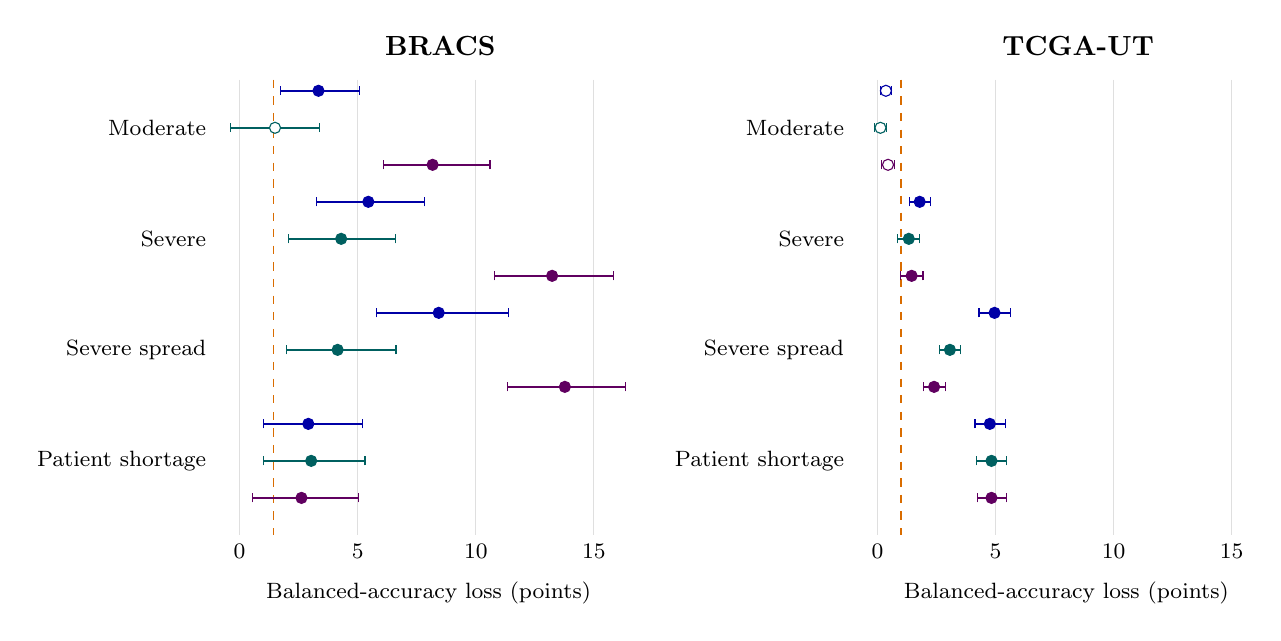
\begin{tikzpicture}[x=0.30cm,y=0.47cm,font=\footnotesize]
\begin{scope}[xshift=0cm]
\node[font=\bfseries] at (8.5,1.2) {BRACS};
\draw[gray!25] (0,0.3)--(0,-12);\node[below] at (0,-12) {0};
\draw[gray!25] (5,0.3)--(5,-12);\node[below] at (5,-12) {5};
\draw[gray!25] (10,0.3)--(10,-12);\node[below] at (10,-12) {10};
\draw[gray!25] (15,0.3)--(15,-12);\node[below] at (15,-12) {15};
\draw[dashed,orange!85!black] (1.443,0.3)--(1.443,-12);
\draw[blue!65!black,thick] (1.72,0)--(5.09,0);\draw[blue!65!black] (1.72,-0.12)--(1.72,0.12) (5.09,-0.12)--(5.09,0.12);
\draw[blue!65!black,fill=blue!65!black] (3.34,0) circle[radius=2pt];
\draw[teal!75!black,thick] (-0.4,-1)--(3.39,-1);\draw[teal!75!black] (-0.4,-1.12)--(-0.4,-0.88) (3.39,-1.12)--(3.39,-0.88);
\draw[teal!75!black,fill=white] (1.5,-1) circle[radius=2pt];
\node[anchor=east,align=right,text width=2.15cm] at (-1,-1) {Moderate};
\draw[violet!75!black,thick] (6.09,-2)--(10.6,-2);\draw[violet!75!black] (6.09,-2.12)--(6.09,-1.88) (10.6,-2.12)--(10.6,-1.88);
\draw[violet!75!black,fill=violet!75!black] (8.17,-2) circle[radius=2pt];
\draw[blue!65!black,thick] (3.27,-3)--(7.8100000000000005,-3);\draw[blue!65!black] (3.27,-3.12)--(3.27,-2.88) (7.8100000000000005,-3.12)--(7.8100000000000005,-2.88);
\draw[blue!65!black,fill=blue!65!black] (5.45,-3) circle[radius=2pt];
\draw[teal!75!black,thick] (2.08,-4)--(6.59,-4);\draw[teal!75!black] (2.08,-4.12)--(2.08,-3.88) (6.59,-4.12)--(6.59,-3.88);
\draw[teal!75!black,fill=teal!75!black] (4.3,-4) circle[radius=2pt];
\node[anchor=east,align=right,text width=2.15cm] at (-1,-4) {Severe};
\draw[violet!75!black,thick] (10.780000000000001,-5)--(15.840000000000002,-5);\draw[violet!75!black] (10.780000000000001,-5.12)--(10.780000000000001,-4.88) (15.840000000000002,-5.12)--(15.840000000000002,-4.88);
\draw[violet!75!black,fill=violet!75!black] (13.23,-5) circle[radius=2pt];
\draw[blue!65!black,thick] (5.79,-6)--(11.37,-6);\draw[blue!65!black] (5.79,-6.12)--(5.79,-5.88) (11.37,-6.12)--(11.37,-5.88);
\draw[blue!65!black,fill=blue!65!black] (8.43,-6) circle[radius=2pt];
\draw[teal!75!black,thick] (1.97,-7)--(6.619999999999999,-7);\draw[teal!75!black] (1.97,-7.12)--(1.97,-6.88) (6.619999999999999,-7.12)--(6.619999999999999,-6.88);
\draw[teal!75!black,fill=teal!75!black] (4.15,-7) circle[radius=2pt];
\node[anchor=east,align=right,text width=2.15cm] at (-1,-7) {Severe spread};
\draw[violet!75!black,thick] (11.33,-8)--(16.34,-8);\draw[violet!75!black] (11.33,-8.12)--(11.33,-7.88) (16.34,-8.12)--(16.34,-7.88);
\draw[violet!75!black,fill=violet!75!black] (13.77,-8) circle[radius=2pt];
\draw[blue!65!black,thick] (1.02,-9)--(5.19,-9);\draw[blue!65!black] (1.02,-9.12)--(1.02,-8.88) (5.19,-9.12)--(5.19,-8.88);
\draw[blue!65!black,fill=blue!65!black] (2.91,-9) circle[radius=2pt];
\draw[teal!75!black,thick] (1.02,-10)--(5.3100000000000005,-10);\draw[teal!75!black] (1.02,-10.12)--(1.02,-9.88) (5.3100000000000005,-10.12)--(5.3100000000000005,-9.88);
\draw[teal!75!black,fill=teal!75!black] (3.0300000000000002,-10) circle[radius=2pt];
\node[anchor=east,align=right,text width=2.15cm] at (-1,-10) {Patient shortage};
\draw[violet!75!black,thick] (0.53,-11)--(5.0200000000000005,-11);\draw[violet!75!black] (0.53,-11.12)--(0.53,-10.88) (5.0200000000000005,-11.12)--(5.0200000000000005,-10.88);
\draw[violet!75!black,fill=violet!75!black] (2.62,-11) circle[radius=2pt];
\node[below] at (8,-13) {Balanced-accuracy loss (points)};
\end{scope}
\begin{scope}[xshift=8.1cm]
\node[font=\bfseries] at (8.5,1.2) {TCGA-UT};
\draw[gray!25] (0,0.3)--(0,-12);\node[below] at (0,-12) {0};
\draw[gray!25] (5,0.3)--(5,-12);\node[below] at (5,-12) {5};
\draw[gray!25] (10,0.3)--(10,-12);\node[below] at (10,-12) {10};
\draw[gray!25] (15,0.3)--(15,-12);\node[below] at (15,-12) {15};
\draw[dashed,orange!85!black] (1,0.3)--(1,-12);
\draw[blue!65!black,thick] (0.12,0)--(0.61,0);\draw[blue!65!black] (0.12,-0.12)--(0.12,0.12) (0.61,-0.12)--(0.61,0.12);
\draw[blue!65!black,fill=white] (0.36,0) circle[radius=2pt];
\draw[teal!75!black,thick] (-0.13,-1)--(0.4,-1);\draw[teal!75!black] (-0.13,-1.12)--(-0.13,-0.88) (0.4,-1.12)--(0.4,-0.88);
\draw[teal!75!black,fill=white] (0.13,-1) circle[radius=2pt];
\node[anchor=east,align=right,text width=2.15cm] at (-1,-1) {Moderate};
\draw[violet!75!black,thick] (0.16999999999999998,-2)--(0.72,-2);\draw[violet!75!black] (0.16999999999999998,-2.12)--(0.16999999999999998,-1.88) (0.72,-2.12)--(0.72,-1.88);
\draw[violet!75!black,fill=white] (0.44999999999999996,-2) circle[radius=2pt];
\draw[blue!65!black,thick] (1.3599999999999999,-3)--(2.23,-3);\draw[blue!65!black] (1.3599999999999999,-3.12)--(1.3599999999999999,-2.88) (2.23,-3.12)--(2.23,-2.88);
\draw[blue!65!black,fill=blue!65!black] (1.79,-3) circle[radius=2pt];
\draw[teal!75!black,thick] (0.86,-4)--(1.79,-4);\draw[teal!75!black] (0.86,-4.12)--(0.86,-3.88) (1.79,-4.12)--(1.79,-3.88);
\draw[teal!75!black,fill=teal!75!black] (1.3299999999999998,-4) circle[radius=2pt];
\node[anchor=east,align=right,text width=2.15cm] at (-1,-4) {Severe};
\draw[violet!75!black,thick] (0.97,-5)--(1.9300000000000002,-5);\draw[violet!75!black] (0.97,-5.12)--(0.97,-4.88) (1.9300000000000002,-5.12)--(1.9300000000000002,-4.88);
\draw[violet!75!black,fill=violet!75!black] (1.4500000000000002,-5) circle[radius=2pt];
\draw[blue!65!black,thick] (4.3,-6)--(5.65,-6);\draw[blue!65!black] (4.3,-6.12)--(4.3,-5.88) (5.65,-6.12)--(5.65,-5.88);
\draw[blue!65!black,fill=blue!65!black] (4.96,-6) circle[radius=2pt];
\draw[teal!75!black,thick] (2.62,-7)--(3.52,-7);\draw[teal!75!black] (2.62,-7.12)--(2.62,-6.88) (3.52,-7.12)--(3.52,-6.88);
\draw[teal!75!black,fill=teal!75!black] (3.0700000000000003,-7) circle[radius=2pt];
\node[anchor=east,align=right,text width=2.15cm] at (-1,-7) {Severe spread};
\draw[violet!75!black,thick] (1.94,-8)--(2.88,-8);\draw[violet!75!black] (1.94,-8.12)--(1.94,-7.88) (2.88,-8.12)--(2.88,-7.88);
\draw[violet!75!black,fill=violet!75!black] (2.4,-8) circle[radius=2pt];
\draw[blue!65!black,thick] (4.130000000000001,-9)--(5.41,-9);\draw[blue!65!black] (4.130000000000001,-9.12)--(4.130000000000001,-8.88) (5.41,-9.12)--(5.41,-8.88);
\draw[blue!65!black,fill=blue!65!black] (4.760000000000001,-9) circle[radius=2pt];
\draw[teal!75!black,thick] (4.21,-10)--(5.46,-10);\draw[teal!75!black] (4.21,-10.12)--(4.21,-9.88) (5.46,-10.12)--(5.46,-9.88);
\draw[teal!75!black,fill=teal!75!black] (4.83,-10) circle[radius=2pt];
\node[anchor=east,align=right,text width=2.15cm] at (-1,-10) {Patient shortage};
\draw[violet!75!black,thick] (4.22,-11)--(5.45,-11);\draw[violet!75!black] (4.22,-11.12)--(4.22,-10.88) (5.45,-11.12)--(5.45,-10.88);
\draw[violet!75!black,fill=violet!75!black] (4.83,-11) circle[radius=2pt];
\node[below] at (8,-13) {Balanced-accuracy loss (points)};
\end{scope}
\end{tikzpicture}

\caption{Patient shortage damages both datasets; moderate patch shortage has a much smaller effect on TCGA-UT. Points and bars show balanced-accuracy deficits and paired 95\% intervals. Within each comparison, rows are native (blue), aligned (teal), and reversed (purple), from top to bottom. Filled points meet both materiality and precision criteria; hollow points do not. Dashed lines mark each dataset's materiality minimum. Both panels use the same horizontal scale. References are concentrated balanced for moderate/severe and balanced spread for severe spread/patient shortage.}
\label{fig:damage-overview}
\end{figure}

\subsection{Probability-quality deficit}
\label{sec:rq1-calibration}
Probability quality measures how much probability the model assigns to the correct class, using tail-group macro negative log likelihood (NLL). For readability, deficits are expressed here as the relative reduction in the geometric-mean probability assigned to the true class. If the NLL increase is $D_{\mathrm{NLL}}$, this reduction is
\begin{equation}
  Q = 100\bigl(1-\exp(-D_{\mathrm{NLL}})\bigr)\%.
\end{equation}
\noindent For example, a \num{20}\% reduction means a reference geometric-mean true-class probability of \num{0.50} would fall to \num{0.40}. This is a relative probability change, not a percentage-point change in accuracy or an arithmetic mean of probabilities. It retains the endpoint's patient, class, and partition weighting. Negative values indicate improvement. The thresholds derived from balanced-condition variation correspond to reductions of \num{13.7}\% on BRACS and \num{5.9}\% on TCGA-UT. The equivalent NLL thresholds are \num{0.14782} and \num{0.06095} \emph{nats}, respectively, where a nat is a natural-log unit. Recovery eligibility still uses the prespecified NLL threshold and a paired \num{95}\% interval excluding zero.

On BRACS, moderate patch shortage reduces geometric-mean true-class probability by \num{17.0}--\num{53.0}\%, severe patch shortage by \num{49.7}--\num{82.5}\%, and severe spread by \num{18.5}--\num{67.7}\%. Native moderate is imprecise, and independent-support reductions of \num{12.5}--\num{13.1}\% fall just below threshold. TCGA-UT differs: moderate patch shortage improves this probability measure, while all three independent-support comparisons reduce it by \num{22.7}--\num{23.1}\%. Among severe concentrated conditions, aligned alone clears threshold; all three severe-spread conditions do. Probability-quality damage therefore depends on dataset and assignment and does not simply follow accuracy damage. Appendix Table~\ref{tab:calibration-deficit} retains the NLL estimates and intervals.

\subsection{Where the damage falls}
\label{sec:rq1-incidence}
Aggregate deficits do not show which support tier absorbs the loss. Table~\ref{tab:tier-endpoints} therefore retains one informative tier for each difficulty-based assignment and dataset; the complete side-by-side tier comparison appears in Appendix~\ref{app:endpoints}. Tier labels in balanced-spread rows reflect class ordering rather than unequal support because that allocation is uniform.

\begin{table}[ht]
  \centering
  \footnotesize
  \resultstable{tier_endpoints_summary}
  \caption{Selected tier recall (\%). Aligned assigns the fewest patches to the hardest classes; reversed assigns those classes the most patches. Head, body, and tail denote high-, intermediate-, and low-support tiers.}
  \label{tab:tier-endpoints}
\end{table}

\noindent BRACS shows substantial tier damage already at moderate severity: aligned tail recall falls from \num{40.9}\% to \num{18.3}\%, while reversed body recall falls from \num{31.2}\% to \num{19.7}\%. TCGA-UT moves less at moderate severity, in line with its sub-threshold aggregate deficit, but severe deprivation lowers aligned tail recall from \num{66.1}\% to \num{51.9}\%. Under the reversed TCGA-UT assignment, severe spread restores head recall to \num{66.4}\%, close to the \num{67.0}\% spread reference. Difficulty and cohort breadth therefore change where damage appears; support rank alone does not identify the affected tier.

\subsection{Natural anchor}
\label{sec:rq1-routing}
The natural condition trains on every eligible patch at each dataset's observed prevalence. It is not size-matched and enters no estimand; it only places the controlled results beside the training distribution encountered without intervention.

\begin{table}[H]
  \centering
  \footnotesize
  \resultstable{natural_anchor_summary}
  \caption{Natural and balanced cross-entropy anchors.}
  \label{tab:natural-anchor}
\end{table}

\noindent On BRACS, natural training uses roughly seven to sixteen times the controlled patch total across partitions yet reaches \num{49.8}\% balanced accuracy, between the concentrated and spread balanced references. On TCGA-UT, the natural anchor reaches \num{79.1}\%, well above the concentrated balanced result of \num{75.3}\% and close to the spread references at \num{79.6}--\num{79.7}\%. The natural anchor therefore reinforces the benefit of broad patient coverage on TCGA-UT but does not isolate it from the much larger patch budget.

\section{Mitigation Recovery}
\label{sec:rq2}
Recovery is defined as $R_M = [M(\text{method}) - M(\text{deprived CE})] / D_M$ and is reported as a percentage of the established deficit. A recovery of \num{0}\% means no improvement over deprived cross-entropy, \num{100}\% reaches the balanced reference, a negative value means further deterioration, and a value above \num{100}\% surpasses the reference. Comparisons that do not meet the materiality and precision criteria in Sections~\ref{sec:rq1-discrimination} and~\ref{sec:rq1-calibration} are omitted because their recovery denominator is not sufficiently stable.

\subsection{Which weighting signals recover discrimination}
\label{sec:rq2-family}
The confirmatory family contains five weighted cross-entropy methods that differ only in the signal used to set their class weights: prevalence, nominal support, independent support, pilot difficulty, or semantic diversity. Each is compared with deprived cross-entropy using a paired permutation test. A result \emph{survives Holm adjustment} when its adjusted $p$-value remains below \num{0.05} after accounting for all confirmatory comparisons, reducing the chance that a result appears significant only because many methods and conditions were tested.

\begin{table}[ht]
  \centering
  \scriptsize
  \setlength{\tabcolsep}{4pt}
  \resultstable{confirmatory_summary}
  \caption{Balanced-accuracy recovery by shortage and weighting signal. Ranges are percentages of the original deficit; the final column counts results that remain significant after Holm adjustment.}
  \label{tab:confirmatory}
\end{table}

\noindent Prevalence and nominal-support weighting are the only signals that repeatedly repair nominal deprivation. On BRACS they recover \num{42.6}--\num{89.2}\% across the eight eligible nominal units, with ten of sixteen comparisons surviving Holm adjustment. TCGA-UT's moderate units do not enter recovery analysis because their deficits are below threshold; across its six severe units, the same two signals recover \num{32.1}--\num{85.3}\% and all six concentrated-severe comparisons survive adjustment. Severe-spread recovery is more mixed: independent-support weighting also recovers \num{8.1}--\num{47.7}\%, and difficulty weighting produces one adjusted deterioration. No weighting repairs independent-support deprivation on either dataset: all estimates lie between $-\num{6.5}$\% and \num{2.5}\% on BRACS and between $-\num{1.9}$\% and \num{0.0}\% on TCGA-UT. Appendix Table~\ref{tab:confirmatory-detail} provides the condition-level estimates and intervals.

Two construction details bound what the difficulty and diversity estimates can mean. Pilot difficulty is frozen from a balanced pilot before the conditions exist, so its weights are identical in every condition and assignment and cannot track the allocation that caused the deficit; because $d_c\in[0,1]$, its weight ratio stays near a factor of two, whereas prevalence and nominal-support weights scale with $\rho=100$. Semantic-scale weighting is estimated on draws with equal cases and patches per class, a deliberate choice that keeps the estimate from encoding prevalence, so it has no direct reading of a nominal shortage. Consistent with this, tuning selected the weakest available difficulty exponent in \num{23} of \num{26} selections, against the strongest available prevalence and nominal-support setting in \num{18} and \num{22}; since the difficulty grid does not contain $\tau=0$, that selection is left-censored. These two arms therefore test two specific weight maps rather than the difficulty and diversity signals themselves.

Figure~\ref{fig:recovery-overview} retains each assignment: the failure to repair patient shortage is shared across signals and datasets, whereas nominal-deprivation recovery varies substantially.

\begin{figure}[p]
\centering
% Generated by assets/build_readable_appendix.mjs; do not edit.
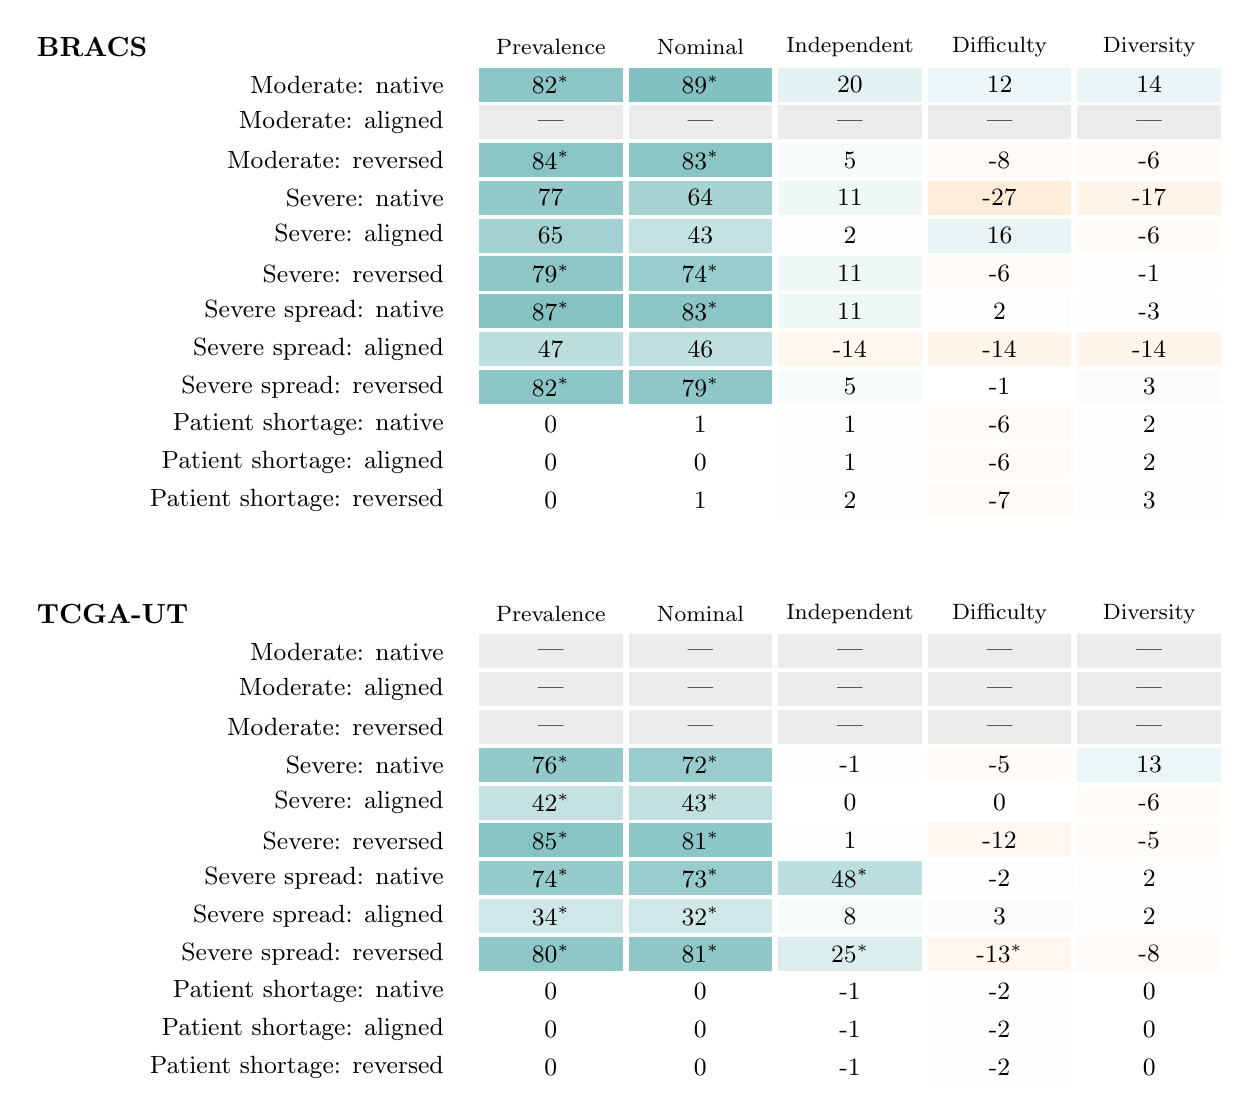
\begin{tikzpicture}[x=1.90cm,y=0.48cm,font=\small]
\node[anchor=west,font=\bfseries] at (-3.5,1) {BRACS};
\node[font=\footnotesize] at (0,1) {Prevalence};
\node[font=\footnotesize] at (1,1) {Nominal};
\node[font=\footnotesize] at (2,1) {Independent};
\node[font=\footnotesize] at (3,1) {Difficulty};
\node[font=\footnotesize] at (4,1) {Diversity};
\node[anchor=east] at (-.65,0) {Moderate: native};
\fill[teal!45!white] (-0.48,-0.45) rectangle (0.48,0.45);\node at (0,0) {82$^{*}$};
\fill[teal!49!white] (0.52,-0.45) rectangle (1.48,0.45);\node at (1,0) {89$^{*}$};
\fill[teal!11!white] (1.52,-0.45) rectangle (2.48,0.45);\node at (2,0) {20};
\fill[teal!7!white] (2.52,-0.45) rectangle (3.48,0.45);\node at (3,0) {12};
\fill[teal!8!white] (3.52,-0.45) rectangle (4.48,0.45);\node at (4,0) {14};
\node[anchor=east] at (-.65,-1) {Moderate: aligned};
\fill[gray!15] (-0.48,-1.45) rectangle (0.48,-0.55);\node at (0,-1) {---};
\fill[gray!15] (0.52,-1.45) rectangle (1.48,-0.55);\node at (1,-1) {---};
\fill[gray!15] (1.52,-1.45) rectangle (2.48,-0.55);\node at (2,-1) {---};
\fill[gray!15] (2.52,-1.45) rectangle (3.48,-0.55);\node at (3,-1) {---};
\fill[gray!15] (3.52,-1.45) rectangle (4.48,-0.55);\node at (4,-1) {---};
\node[anchor=east] at (-.65,-2) {Moderate: reversed};
\fill[teal!46!white] (-0.48,-2.45) rectangle (0.48,-1.55);\node at (0,-2) {84$^{*}$};
\fill[teal!46!white] (0.52,-2.45) rectangle (1.48,-1.55);\node at (1,-2) {83$^{*}$};
\fill[teal!3!white] (1.52,-2.45) rectangle (2.48,-1.55);\node at (2,-2) {5};
\fill[orange!4!white] (2.52,-2.45) rectangle (3.48,-1.55);\node at (3,-2) {-8};
\fill[orange!4!white] (3.52,-2.45) rectangle (4.48,-1.55);\node at (4,-2) {-6};
\node[anchor=east] at (-.65,-3) {Severe: native};
\fill[teal!42!white] (-0.48,-3.45) rectangle (0.48,-2.55);\node at (0,-3) {77};
\fill[teal!35!white] (0.52,-3.45) rectangle (1.48,-2.55);\node at (1,-3) {64};
\fill[teal!6!white] (1.52,-3.45) rectangle (2.48,-2.55);\node at (2,-3) {11};
\fill[orange!15!white] (2.52,-3.45) rectangle (3.48,-2.55);\node at (3,-3) {-27};
\fill[orange!9!white] (3.52,-3.45) rectangle (4.48,-2.55);\node at (4,-3) {-17};
\node[anchor=east] at (-.65,-4) {Severe: aligned};
\fill[teal!36!white] (-0.48,-4.45) rectangle (0.48,-3.55);\node at (0,-4) {65};
\fill[teal!23!white] (0.52,-4.45) rectangle (1.48,-3.55);\node at (1,-4) {43};
\fill[teal!1!white] (1.52,-4.45) rectangle (2.48,-3.55);\node at (2,-4) {2};
\fill[teal!9!white] (2.52,-4.45) rectangle (3.48,-3.55);\node at (3,-4) {16};
\fill[orange!3!white] (3.52,-4.45) rectangle (4.48,-3.55);\node at (4,-4) {-6};
\node[anchor=east] at (-.65,-5) {Severe: reversed};
\fill[teal!44!white] (-0.48,-5.45) rectangle (0.48,-4.55);\node at (0,-5) {79$^{*}$};
\fill[teal!40!white] (0.52,-5.45) rectangle (1.48,-4.55);\node at (1,-5) {74$^{*}$};
\fill[teal!6!white] (1.52,-5.45) rectangle (2.48,-4.55);\node at (2,-5) {11};
\fill[orange!3!white] (2.52,-5.45) rectangle (3.48,-4.55);\node at (3,-5) {-6};
\fill[orange!1!white] (3.52,-5.45) rectangle (4.48,-4.55);\node at (4,-5) {-1};
\node[anchor=east] at (-.65,-6) {Severe spread: native};
\fill[teal!48!white] (-0.48,-6.45) rectangle (0.48,-5.55);\node at (0,-6) {87$^{*}$};
\fill[teal!46!white] (0.52,-6.45) rectangle (1.48,-5.55);\node at (1,-6) {83$^{*}$};
\fill[teal!6!white] (1.52,-6.45) rectangle (2.48,-5.55);\node at (2,-6) {11};
\fill[teal!1!white] (2.52,-6.45) rectangle (3.48,-5.55);\node at (3,-6) {2};
\fill[orange!1!white] (3.52,-6.45) rectangle (4.48,-5.55);\node at (4,-6) {-3};
\node[anchor=east] at (-.65,-7) {Severe spread: aligned};
\fill[teal!26!white] (-0.48,-7.45) rectangle (0.48,-6.55);\node at (0,-7) {47};
\fill[teal!25!white] (0.52,-7.45) rectangle (1.48,-6.55);\node at (1,-7) {46};
\fill[orange!7!white] (1.52,-7.45) rectangle (2.48,-6.55);\node at (2,-7) {-14};
\fill[orange!8!white] (2.52,-7.45) rectangle (3.48,-6.55);\node at (3,-7) {-14};
\fill[orange!8!white] (3.52,-7.45) rectangle (4.48,-6.55);\node at (4,-7) {-14};
\node[anchor=east] at (-.65,-8) {Severe spread: reversed};
\fill[teal!45!white] (-0.48,-8.45) rectangle (0.48,-7.55);\node at (0,-8) {82$^{*}$};
\fill[teal!44!white] (0.52,-8.45) rectangle (1.48,-7.55);\node at (1,-8) {79$^{*}$};
\fill[teal!3!white] (1.52,-8.45) rectangle (2.48,-7.55);\node at (2,-8) {5};
\fill[orange!0!white] (2.52,-8.45) rectangle (3.48,-7.55);\node at (3,-8) {-1};
\fill[teal!2!white] (3.52,-8.45) rectangle (4.48,-7.55);\node at (4,-8) {3};
\node[anchor=east] at (-.65,-9) {Patient shortage: native};
\fill[teal!0!white] (-0.48,-9.45) rectangle (0.48,-8.55);\node at (0,-9) {0};
\fill[teal!0!white] (0.52,-9.45) rectangle (1.48,-8.55);\node at (1,-9) {1};
\fill[teal!1!white] (1.52,-9.45) rectangle (2.48,-8.55);\node at (2,-9) {1};
\fill[orange!3!white] (2.52,-9.45) rectangle (3.48,-8.55);\node at (3,-9) {-6};
\fill[teal!1!white] (3.52,-9.45) rectangle (4.48,-8.55);\node at (4,-9) {2};
\node[anchor=east] at (-.65,-10) {Patient shortage: aligned};
\fill[teal!0!white] (-0.48,-10.45) rectangle (0.48,-9.55);\node at (0,-10) {0};
\fill[teal!0!white] (0.52,-10.45) rectangle (1.48,-9.55);\node at (1,-10) {0};
\fill[teal!1!white] (1.52,-10.45) rectangle (2.48,-9.55);\node at (2,-10) {1};
\fill[orange!3!white] (2.52,-10.45) rectangle (3.48,-9.55);\node at (3,-10) {-6};
\fill[teal!1!white] (3.52,-10.45) rectangle (4.48,-9.55);\node at (4,-10) {2};
\node[anchor=east] at (-.65,-11) {Patient shortage: reversed};
\fill[teal!0!white] (-0.48,-11.45) rectangle (0.48,-10.55);\node at (0,-11) {0};
\fill[teal!0!white] (0.52,-11.45) rectangle (1.48,-10.55);\node at (1,-11) {1};
\fill[teal!1!white] (1.52,-11.45) rectangle (2.48,-10.55);\node at (2,-11) {2};
\fill[orange!4!white] (2.52,-11.45) rectangle (3.48,-10.55);\node at (3,-11) {-7};
\fill[teal!1!white] (3.52,-11.45) rectangle (4.48,-10.55);\node at (4,-11) {3};
\node[anchor=west,font=\bfseries] at (-3.5,-14) {TCGA-UT};
\node[font=\footnotesize] at (0,-14) {Prevalence};
\node[font=\footnotesize] at (1,-14) {Nominal};
\node[font=\footnotesize] at (2,-14) {Independent};
\node[font=\footnotesize] at (3,-14) {Difficulty};
\node[font=\footnotesize] at (4,-14) {Diversity};
\node[anchor=east] at (-.65,-15) {Moderate: native};
\fill[gray!15] (-0.48,-15.45) rectangle (0.48,-14.55);\node at (0,-15) {---};
\fill[gray!15] (0.52,-15.45) rectangle (1.48,-14.55);\node at (1,-15) {---};
\fill[gray!15] (1.52,-15.45) rectangle (2.48,-14.55);\node at (2,-15) {---};
\fill[gray!15] (2.52,-15.45) rectangle (3.48,-14.55);\node at (3,-15) {---};
\fill[gray!15] (3.52,-15.45) rectangle (4.48,-14.55);\node at (4,-15) {---};
\node[anchor=east] at (-.65,-16) {Moderate: aligned};
\fill[gray!15] (-0.48,-16.45) rectangle (0.48,-15.55);\node at (0,-16) {---};
\fill[gray!15] (0.52,-16.45) rectangle (1.48,-15.55);\node at (1,-16) {---};
\fill[gray!15] (1.52,-16.45) rectangle (2.48,-15.55);\node at (2,-16) {---};
\fill[gray!15] (2.52,-16.45) rectangle (3.48,-15.55);\node at (3,-16) {---};
\fill[gray!15] (3.52,-16.45) rectangle (4.48,-15.55);\node at (4,-16) {---};
\node[anchor=east] at (-.65,-17) {Moderate: reversed};
\fill[gray!15] (-0.48,-17.45) rectangle (0.48,-16.55);\node at (0,-17) {---};
\fill[gray!15] (0.52,-17.45) rectangle (1.48,-16.55);\node at (1,-17) {---};
\fill[gray!15] (1.52,-17.45) rectangle (2.48,-16.55);\node at (2,-17) {---};
\fill[gray!15] (2.52,-17.45) rectangle (3.48,-16.55);\node at (3,-17) {---};
\fill[gray!15] (3.52,-17.45) rectangle (4.48,-16.55);\node at (4,-17) {---};
\node[anchor=east] at (-.65,-18) {Severe: native};
\fill[teal!42!white] (-0.48,-18.45) rectangle (0.48,-17.55);\node at (0,-18) {76$^{*}$};
\fill[teal!40!white] (0.52,-18.45) rectangle (1.48,-17.55);\node at (1,-18) {72$^{*}$};
\fill[orange!1!white] (1.52,-18.45) rectangle (2.48,-17.55);\node at (2,-18) {-1};
\fill[orange!3!white] (2.52,-18.45) rectangle (3.48,-17.55);\node at (3,-18) {-5};
\fill[teal!7!white] (3.52,-18.45) rectangle (4.48,-17.55);\node at (4,-18) {13};
\node[anchor=east] at (-.65,-19) {Severe: aligned};
\fill[teal!23!white] (-0.48,-19.45) rectangle (0.48,-18.55);\node at (0,-19) {42$^{*}$};
\fill[teal!24!white] (0.52,-19.45) rectangle (1.48,-18.55);\node at (1,-19) {43$^{*}$};
\fill[orange!0!white] (1.52,-19.45) rectangle (2.48,-18.55);\node at (2,-19) {0};
\fill[teal!0!white] (2.52,-19.45) rectangle (3.48,-18.55);\node at (3,-19) {0};
\fill[orange!3!white] (3.52,-19.45) rectangle (4.48,-18.55);\node at (4,-19) {-6};
\node[anchor=east] at (-.65,-20) {Severe: reversed};
\fill[teal!47!white] (-0.48,-20.45) rectangle (0.48,-19.55);\node at (0,-20) {85$^{*}$};
\fill[teal!45!white] (0.52,-20.45) rectangle (1.48,-19.55);\node at (1,-20) {81$^{*}$};
\fill[teal!1!white] (1.52,-20.45) rectangle (2.48,-19.55);\node at (2,-20) {1};
\fill[orange!6!white] (2.52,-20.45) rectangle (3.48,-19.55);\node at (3,-20) {-12};
\fill[orange!3!white] (3.52,-20.45) rectangle (4.48,-19.55);\node at (4,-20) {-5};
\node[anchor=east] at (-.65,-21) {Severe spread: native};
\fill[teal!41!white] (-0.48,-21.45) rectangle (0.48,-20.55);\node at (0,-21) {74$^{*}$};
\fill[teal!40!white] (0.52,-21.45) rectangle (1.48,-20.55);\node at (1,-21) {73$^{*}$};
\fill[teal!26!white] (1.52,-21.45) rectangle (2.48,-20.55);\node at (2,-21) {48$^{*}$};
\fill[orange!1!white] (2.52,-21.45) rectangle (3.48,-20.55);\node at (3,-21) {-2};
\fill[teal!1!white] (3.52,-21.45) rectangle (4.48,-20.55);\node at (4,-21) {2};
\node[anchor=east] at (-.65,-22) {Severe spread: aligned};
\fill[teal!19!white] (-0.48,-22.45) rectangle (0.48,-21.55);\node at (0,-22) {34$^{*}$};
\fill[teal!18!white] (0.52,-22.45) rectangle (1.48,-21.55);\node at (1,-22) {32$^{*}$};
\fill[teal!4!white] (1.52,-22.45) rectangle (2.48,-21.55);\node at (2,-22) {8};
\fill[teal!2!white] (2.52,-22.45) rectangle (3.48,-21.55);\node at (3,-22) {3};
\fill[teal!1!white] (3.52,-22.45) rectangle (4.48,-21.55);\node at (4,-22) {2};
\node[anchor=east] at (-.65,-23) {Severe spread: reversed};
\fill[teal!44!white] (-0.48,-23.45) rectangle (0.48,-22.55);\node at (0,-23) {80$^{*}$};
\fill[teal!44!white] (0.52,-23.45) rectangle (1.48,-22.55);\node at (1,-23) {81$^{*}$};
\fill[teal!14!white] (1.52,-23.45) rectangle (2.48,-22.55);\node at (2,-23) {25$^{*}$};
\fill[orange!7!white] (2.52,-23.45) rectangle (3.48,-22.55);\node at (3,-23) {-13$^{*}$};
\fill[orange!4!white] (3.52,-23.45) rectangle (4.48,-22.55);\node at (4,-23) {-8};
\node[anchor=east] at (-.65,-24) {Patient shortage: native};
\fill[orange!0!white] (-0.48,-24.45) rectangle (0.48,-23.55);\node at (0,-24) {0};
\fill[teal!0!white] (0.52,-24.45) rectangle (1.48,-23.55);\node at (1,-24) {0};
\fill[orange!0!white] (1.52,-24.45) rectangle (2.48,-23.55);\node at (2,-24) {-1};
\fill[orange!1!white] (2.52,-24.45) rectangle (3.48,-23.55);\node at (3,-24) {-2};
\fill[orange!0!white] (3.52,-24.45) rectangle (4.48,-23.55);\node at (4,-24) {0};
\node[anchor=east] at (-.65,-25) {Patient shortage: aligned};
\fill[orange!0!white] (-0.48,-25.45) rectangle (0.48,-24.55);\node at (0,-25) {0};
\fill[teal!0!white] (0.52,-25.45) rectangle (1.48,-24.55);\node at (1,-25) {0};
\fill[orange!0!white] (1.52,-25.45) rectangle (2.48,-24.55);\node at (2,-25) {-1};
\fill[orange!1!white] (2.52,-25.45) rectangle (3.48,-24.55);\node at (3,-25) {-2};
\fill[orange!0!white] (3.52,-25.45) rectangle (4.48,-24.55);\node at (4,-25) {0};
\node[anchor=east] at (-.65,-26) {Patient shortage: reversed};
\fill[orange!0!white] (-0.48,-26.45) rectangle (0.48,-25.55);\node at (0,-26) {0};
\fill[teal!0!white] (0.52,-26.45) rectangle (1.48,-25.55);\node at (1,-26) {0};
\fill[orange!0!white] (1.52,-26.45) rectangle (2.48,-25.55);\node at (2,-26) {-1};
\fill[orange!1!white] (2.52,-26.45) rectangle (3.48,-25.55);\node at (3,-26) {-2};
\fill[orange!0!white] (3.52,-26.45) rectangle (4.48,-25.55);\node at (4,-26) {0};
\end{tikzpicture}

\caption{Weighting repairs nominal deprivation more readily than patient shortage. Cells show balanced-accuracy recovery (\%), rounded to whole percentages: 0 means no repair and 100 reaches the balanced reference. Teal indicates improvement and orange deterioration; colour intensity saturates at an absolute recovery of 100\%, while numbers remain untruncated. Asterisks mark Holm-adjusted $p<0.05$ from the permutation tests; paired intervals appear in Appendix~\ref{app:recovery-estimates}. Grey dashes mean the original deficit is ineligible, not zero recovery. Columns denote the five weighting signals, with nominal and independent referring to support.}
\label{fig:recovery-overview}
\end{figure}

\subsection{Matched against unmatched signals}
\label{sec:rq2-matched}
A method is \emph{matched} when its weighting signal corresponds to the dominant shortage identified for that condition in Table~\ref{tab:signal-profiles}; for example, independent-support weighting is matched to a condition that reduces patient breadth. The unmatched arm contains the other weighting signals. Conditions without one clear dominant shortage are excluded from this contrast. A positive matched-minus-unmatched value therefore favours the signal selected by the condition profile.

\begin{table}[ht]
  \centering
  \small
  \resultstable{matched_contrast_summary}
  \caption{Matched-minus-unmatched contrasts for balanced accuracy. Intervals are paired \num{95}\% bootstrap intervals.}
  \label{tab:matched-contrast}
\end{table}

\noindent For independent-support deprivation, matched weighting changes balanced accuracy by only \num{0.06} percentage points on BRACS and \num{0.00} on TCGA-UT; both intervals cover zero. Matching favours the corresponding signal in the two BRACS nominal-support units and the one TCGA-UT nominal-support unit. When difficulty or diversity is dominant, the matched method never outperforms the effective prevalence-based alternatives and is worse in two units. Those units are patch-shortage conditions: dominance is assigned from standardized scores, and no condition creates a difficulty or diversity shortage while holding patch counts fixed. The contrast therefore compares weighting rules within a nominal deprivation.

Both independent-support and class-balanced weighting use an effective-number formula whose parameter $\beta$ controls weight strength. The matched-$\beta$ diagnostic gives independent-support weighting the value selected for class-balanced cross-entropy, separating the count source from tuning strength. It does not alter the conclusion on either dataset. Full matched contrasts and matched-$\beta$ results appear in Appendix Tables~\ref{tab:matched-contrast-detail} and~\ref{tab:matched-beta-detail}.

\subsection{Recovery of probability quality}
\label{sec:rq2-calibration}
A method can restore balanced accuracy while making its probabilities worse. The prespecified recovery endpoint is tail-group macro negative log likelihood computed from raw test probabilities; temperature scaling never enters the confirmatory decisions. Recovery is analysed only where the dataset-specific raw-score deficit is sufficiently large and precise.

\begin{table}[ht]
  \centering
  \small
  \resultstable{calibration_recovery_summary}
  \caption{Recovery of tail-group probability quality. Recovery is the percentage of the original negative-log-likelihood deficit.}
  \label{tab:calibration-recovery}
\end{table}

\noindent On BRACS, prevalence and nominal-support weighting improve raw probability quality in seven of eight eligible units, whereas the other three signals deteriorate in all \num{24} comparisons. TCGA-UT does not repeat that simple pattern. All five signals worsen the three independent-support units by \num{51.7}--\num{62.4}\% of the original deficit, while prevalence and nominal-support weighting recover \num{106.5}\% and \num{92.2}\% in aligned concentrated severe. Across severe-spread assignments the result changes from improvement to mixed response to deterioration. Probability-quality recovery is therefore conditional on dataset and assignment even when discrimination recovery is consistent. Exact intervals and adjusted $p$-values appear in Appendix Table~\ref{tab:calibration-recovery-detail}; Appendix~\ref{app:calibration} gives the full temperature-scaling analysis summarized below.

Temperature scaling fits a single confidence adjustment on validation data and leaves predicted classes unchanged. Repeating the tail-group contrasts after scaling removes much of the nominal-deprivation effect: among the raw-eligible nominal comparisons, three of eight BRACS deficits and two of four TCGA-UT deficits still exceed their dataset's magnitude threshold. Some nominal deficits change sign, including aligned severe on TCGA-UT. Patient shortage behaves differently. TCGA-UT's geometric-mean true-class probability remains \num{20.4}--\num{20.7}\% below its spread reference after scaling, compared with \num{22.7}--\num{23.1}\% before scaling; all three paired intervals still exclude zero. On BRACS, the corresponding deficit decreases from \num{12.5}--\num{13.1}\% before scaling to \num{9.7}--\num{10.3}\% after scaling. Scaling therefore reduces the independent-support deficit but does not eliminate its positive point estimate. Both ranges are below BRACS's \num{13.7}\% materiality threshold; being below that threshold does not mean that the deficit is zero. Nor does scaling eliminate all BRACS probability-quality deficits: reversed severe, reversed severe spread, and aligned severe spread retain deficits above the magnitude threshold.

The apparent probability-quality benefit of prevalence and nominal-support weighting largely disappears after scaling. On BRACS, the number of improvements with intervals excluding zero falls from fourteen of sixteen comparisons to one, and four estimates change to deterioration. On TCGA-UT, all fourteen comparisons for these two methods become deteriorations with intervals excluding zero. Independent-support, difficulty, and diversity weighting also retain deterioration in every evaluated comparison, although scaling reduces its magnitude. Thus TCGA-UT's scaled method effects have a consistent direction across assignments: none of the five weighting signals improves probability quality relative to scaled deprived cross-entropy. This directional consistency concerns mitigation effects; it does not mean every allocation-induced deficit has the same sign. Scaled contrasts are exploratory paired-bootstrap results, without the confirmatory permutation tests or multiplicity adjustment used for the raw endpoint.

\subsection{Exploratory methods beyond weighting}
\label{sec:rq2-roster}
The wider roster varies the training objective, sampling distribution, decision rule, or classifier head. Its estimates are exploratory because methods no longer differ by signal alone; several also reduce to the same balanced-sampling mechanism and should not be read as independent confirmations.

\begin{table}[ht]
  \centering
  \small
  \resultstable{roster_recovery_summary}
  \caption{Most informative recovery results from the exploratory method roster.}
  \label{tab:roster-recovery}
\end{table}

\noindent The roster confirms that severe nominal-support deficits are broadly repairable: the best estimates are \num{55.4}--\num{90.8}\% on BRACS and \num{90.0}--\num{130.6}\% on TCGA-UT. Independent-support damage remains largely unrecovered. No BRACS method has positive recovery with an interval excluding zero. TCGA-UT's CFAL and OKO estimates are positive but close only \num{12.9}--\num{16.6}\% of the deficit, while classifier retraining deteriorates by about \num{13.5}\%. Thus no tested method closes a substantial share of the independent-support loss.

The roster also separates signal from mechanism on the nominal axis. Focal loss and CFAL read example difficulty and recover \num{38}--\num{108}\% of the severe concentrated deficits, against $-\num{27}$--\num{16}\% for difficulty weighting on the same units. Both couple difficulty with prevalence or nominal support, so this does not isolate difficulty; it does show that difficulty-sensitive mechanisms repair deficits a static class-difficulty weight leaves in place. No roster method reads a diversity signal, so diversity has no second reading. Full method-level estimates appear in Appendix Table~\ref{tab:roster-recovery-detail}.

\section{Explaining Heterogeneity}
\label{sec:rq3}
Damage magnitude and recovery headroom vary across conditions, and RQ3 asks which realized shortages track that variation. Two association models are specified, one for signed balanced-accuracy damage over the cross-entropy cells and one for recovery over the gate-passing method cells. Both use the same linear predictor over standardized quantities,
\begin{equation}
  \mu_j = \alpha + u_{g[j]} + \beta_{\rho}\log \rho_j + \beta_{\mathrm{ind}} S_{\mathrm{ind},j} + \beta_{A} A_j + \beta_{\mathrm{div}} S_{\mathrm{div},j},
  \label{eq:rq3-model}
\end{equation}
\noindent where $\rho_j$ is achieved severity, $S_{\mathrm{ind},j}$ the independent-support shortage, $A_j$ the support--difficulty alignment, $S_{\mathrm{div},j}$ the diversity shortage, and $u_{g[j]}$ a random intercept over dataset--target groups that absorbs level differences between datasets. Observation errors come from the bootstrap distributions of the corresponding endpoints.

The fitted sample consists of BRACS and TCGA-UT. For each model, predictors are centered and divided by their standard deviations across the observations entering that fit. These model scales differ from the within-dataset shortage scores used to select matched methods in Table~\ref{tab:signal-profiles}. Each coefficient describes the change associated with a one-standard-deviation increase in its predictor, holding the other predictors fixed.

\begin{table}[ht]
  \centering
  \scriptsize
  \resultstable{rq3_models}
  \caption{Maximum a posteriori estimates for the two exploratory association models fitted to BRACS and TCGA-UT. Damage is signed balanced-accuracy loss and recovery is the recovered fraction. Predictors are standardized within each model's fitted sample.}
  \label{tab:rq3-models}
\end{table}

\noindent Conditional on the other profile variables, achieved severity and independent-support shortage have positive damage coefficients, \num{0.0318} and \num{0.0158}. In the recovery model, independent-support shortage has the largest coefficient in magnitude and is negative, $-\num{0.3385}$; severity is also negative, while alignment and diversity are small and positive. The damage model's diversity coefficient is small and negative, reversing the expected direction; the model conditions on achieved severity rather than nominal shortage while $S_{\mathrm{div}}$ moves with the patch allocation, so it should not be read as a protective effect of low diversity. These are exploratory associations, not causal effects, and two dataset--target groups cannot establish that the coefficients transport to a new dataset.

Prediction on an unseen dataset is examined in Appendix~\ref{app:rq3-prediction}.

\section{Discussion}
\label{sec:discussion}
The preceding sections establish what the controlled allocations damaged and how much of that damage the tested methods returned. This section reads those outcomes as design evidence. The question is not which existing method won, but what a mitigation method would have to read and do across two distinct evidence regimes.

\subsection{What the evidence supports}
\label{sec:discussion-evidence}
RQ1 separates nominal patch shortage from independent patient shortage on both datasets. Moderate nominal deprivation is material on BRACS but not TCGA-UT, showing that severity labels do not imply equal damage across datasets. Severe deprivation damages both, with assignment determining which tier is affected. Independent-support deprivation replicates more strongly: holding patches fixed costs \num{2.62}--\num{3.03} balanced-accuracy points on BRACS and \num{4.76}--\num{4.83} on TCGA-UT. Patch count alone therefore does not characterize whether a class has enough independent training evidence.

Two hypotheses could explain BRACS's greater sensitivity to moderate patch shortage. First, the same largest-to-smallest class ratio redistributes class shares differently in a seven-class and a thirty-class task: at moderate severity, the entropy deficit is \num{0.128} on BRACS but \num{0.061} on TCGA-UT. The ratio therefore does not represent an equal overall disruption. Second, BRACS may have less margin for removing examples from difficult classes. Its aligned tail recall already starts at \num{40.9}\% in the balanced reference, compared with \num{66.1}\% on TCGA-UT, and its controlled patient pool is much smaller. One possibility is that frozen features separate BRACS lesion classes less well, making missing examples more consequential. These are hypotheses rather than identified causes: task, class structure, patient coverage, and feature suitability vary together. They could be tested by matching per-class patient support and class-share disruption across tasks, then comparing damage against pilot class difficulty. TCGA-UT's sub-threshold moderate result should not be read as evidence that moderate imbalance is harmless in general.

RQ2 shows that prevalence and nominal-support weighting repair much of the severe discrimination deficit on both datasets, as do several roster mechanisms reading other signals. No weighting repairs independent-support discrimination damage, and widening the mechanism roster closes at most about one sixth of TCGA-UT's deficit. A plausible explanation is that class weighting changes the influence of observed patches but cannot supply patient variation absent from training. This interpretation motivates testing methods that broaden patient sampling or explicitly account for repeated patches from the same patient.

Temperature-scaled probabilities give the clearer interpretation of TCGA-UT's mitigation results. The assignment-dependent improvements and deteriorations on raw probabilities become consistent deterioration across the five weighting signals after confidence adjustment. Much of the raw benefit from prevalence-based weighting therefore appears to correct confidence scale rather than add probability-quality benefit beyond temperature scaling. Yet patient shortage still reduces geometric-mean true-class probability by about \num{20}\% after scaling, suggesting that this loss cannot be explained by a single confidence-scale error. On BRACS, most prevalence-based benefits also disappear, but allocation-induced damage remains: the patient-shortage deficit is reduced to about \num{10}\%, not eliminated, and three nominal-deprivation comparisons retain deficits above the materiality threshold. BRACS's patient-shortage deficit was below threshold before scaling as well. Calibration thus clarifies TCGA-UT's method comparison without making all allocation effects uniform. This interpretation is exploratory, and the methods were tuned for balanced accuracy rather than NLL; it does not establish that probability-focused tuning would fail (Section~\ref{sec:rq2-calibration} and Appendix~\ref{app:calibration}).

RQ3 is consistent with these controlled contrasts: severity and independent shortage are positively associated with damage, and independent shortage is negatively associated with recovery after conditioning on the remaining profile. The fit is exploratory: BRACS and TCGA-UT provide two dataset--target groups. These associations motivate hypotheses rather than transferable prediction rules.

\subsection{Which shortage a mitigation method must read}
\label{sec:discussion-signal}
A method must estimate the shortage that binds, but reading the correct count is useful only if its intervention can address that shortage. The patient-shortage comparison changes patient coverage while keeping each class's patch count fixed. This produces a precise deficit at both the weaker BRACS dose and the stronger TCGA-UT dose, yet independent-support weighting remains near zero recovery in both. The result is therefore not explained by an inactive manipulation or a single dataset's dose.

All five confirmatory members apply a per-class scalar to the loss. Such a scalar can emphasize examples but cannot add independent observations. When many patches come from few patients, stronger emphasis may instead amplify patient-specific regularities. A method aimed at independent shortage therefore needs a different mechanism, such as patient-level aggregation or information sharing, and must be tested while patient breadth varies independently of patch count.

\subsection{Signal against mechanism}
\label{sec:discussion-mechanism}
The confirmatory family shares one intervention mechanism, so on the nominal axis it compares weight maps: prevalence and nominal support outperform the difficulty and diversity weights on both datasets. That result is about the weighting rules, not about the underlying signals. The roster separates the two levels, and the separation matters most for difficulty: focal loss and CFAL act on the same signal through a dynamic, example-level mechanism and recover much of the severe nominal deficit, so the failure of difficulty weighting is a failure of a frozen per-class weight rather than of difficulty as a mitigation signal. Diversity admits no such comparison, since no roster method reads it.

On the independent axis the levels agree. Changing the signal does not help, and changing the mechanism helps little: the roster finds no meaningful BRACS recovery and only \num{12.9}--\num{16.6}\% recovery from TCGA-UT's best two methods. This small nonzero result rules out the stronger claim that every wider-roster estimate is null, but it does not close a substantial share of the deficit.

\subsection{Where tested methods reach a ceiling}
\label{sec:discussion-ceiling}
Existing mechanisms recover most severe nominal damage, so a new method is not justified by that regime alone. The unmet need is independent patient support: its discrimination damage replicates, grows under TCGA-UT's stronger contrast, and remains mostly unrecovered. The complementary finding is that intervention should be conditional. TCGA-UT's moderate allocation is nominally imbalanced but produces no material discrimination deficit, and probability-quality effects change direction across datasets and assignments. Applying mitigation whenever a count ratio looks large risks treating damage that is absent or worsening an endpoint that was not the target.

\subsection{Design requirements and open questions}
\label{sec:discussion-requirements}
The replicated and dataset-dependent findings resolve into four requirements:
\begin{enumerate}
  \item Diagnose material damage, not imbalance ratio alone; moderate BRACS and TCGA-UT allocations demonstrate that the same nominal severity can have different consequences.
  \item Use prevalence or nominal support for class weighting when severe nominal deprivation damages discrimination. The frozen class-difficulty and semantic-scale weight maps tested here are not effective substitutes, but that finding concerns those weighting rules: methods reading example difficulty through a dynamic mechanism recover comparable deficits, and the diversity axis was never manipulated.
  \item Address independent-support shortage with a mechanism beyond per-class weights, and evaluate it at patient level while patch totals remain fixed.
  \item Judge discrimination and probability quality separately, including after validation-fitted calibration, and remain inactive when the target deficit is absent.
\end{enumerate}
\noindent A focused next experiment should therefore hold patch counts fixed while varying patient breadth and within-patient redundancy, then test a patient-aware objective rather than another per-class weight. A patient-macro objective, which averages patch losses within each patient before weighting patients equally, is the simplest candidate. Hierarchical sharing across patients or classes is a more complex alternative. The RQ3 coefficients can prioritize hypotheses, but their two-group fit is not strong enough to select a mechanism by itself.

\section{Conclusion and Scope}
\label{sec:limits}
Across BRACS and TCGA-UT, controlled allocation separates two effects that ordinary imbalance confounds. Severe nominal patch deprivation is largely repairable through prevalence or nominal-support weighting. Independent patient deprivation damages discrimination even when patch allocation is unchanged, and no tested class weighting repairs it; the wider roster closes at most a small share. Calibration effects vary across datasets and assignments, and post-hoc temperature scaling reduces many nominal-allocation effects but does not eliminate every BRACS deficit. Independent-support deficit estimates remain positive on both datasets; BRACS stays below its materiality threshold, while TCGA-UT remains above its threshold. The exploratory RQ3 fit agrees with the controlled comparisons but remains hypothesis-generating. Together these results motivate patient-aware mitigation that diagnoses damage before acting and evaluates probability quality separately from discrimination.

Four conditions bound the claims. Each dataset's three partitions are repeated partitions, not independent cohorts, so intervals do not measure variation across populations. Within a dataset, the three independent-support units share one deprived allocation and differ only in reference assignment, so the two datasets provide the replications, not the three assignments. The benchmark covers patch classification only; at whole-slide level, reallocating labelled slides changes nominal and independent support together. Temperature scaling is a diagnostic and never determines the confirmatory recovery analysis. Finally, only nominal and independent support are manipulated: difficulty enters through the support--difficulty assignment and diversity only as a realized description, so claims about either signal are limited to the weighting rules that were tested.

\newpage
\appendix
\phantomsection
\addcontentsline{toc}{part}{Appendices}
\addtocontents{toc}{\protect\setcounter{tocdepth}{1}}

\section{What Was Held Fixed, and What Was Checked}
\label{app:realized}
The supporting analyses address four questions: whether the intended allocations were achieved, whether the estimates have adequate patient support, whether recovery depends on the assignment, and whether calibration or partition variation changes the interpretation. Repeated execution records are summarized as ranges; paired uncertainty intervals are retained for the primary damage and weighting comparisons. Ranges describe observed variation, not confidence intervals.

\subsection{Allocation and patient coverage}
\label{app:realized-construction}
Table~\ref{tab:realized-support} separates class imbalance from patient coverage. Within each partition, balanced and balanced-spread training use identical class-specific patch counts. Their patient counts differ substantially, especially on TCGA-UT. Moderate and severe allocations meet their target ratios of 9--11 and 90--110, respectively; none is off-target or collapses to balance. Small departures from a ratio of one in balanced training reflect integer allocation.

\begin{table}[H]
\centering\footnotesize\setlength{\tabcolsep}{3pt}
% Generated by assets/build_readable_appendix.mjs; do not edit.
\begin{tabular}{@{}lrrrr@{}}
\toprule
Allocation & Patients & Patches & $\rho$ & $1-H_{\rm norm}$ \\
\midrule
\multicolumn{5}{@{}l}{\textbf{BRACS}} \\
Natural & \num{103} & \num{193010} to \num{217704} & \num{5.722} to \num{8.297} & \num{0.1178} to \num{0.1432} \\
Balanced & \num{78} to \num{89} & \num{13982} to \num{27202} & \num{1.000} to \num{1.001} & \num{0.0000} \\
Balanced spread & \num{103} & \num{13982} to \num{27202} & \num{1.000} to \num{1.001} & \num{0.0000} \\
Moderate & \num{78} to \num{89} & \num{13982} to \num{27202} & \num{10.003} to \num{10.007} & \num{0.1280} \\
Severe & \num{78} to \num{89} & \num{13982} to \num{27202} & \num{100.301} to \num{100.467} & \num{0.3530} \\
Severe spread & \num{103} & \num{13982} to \num{27202} & \num{100.301} to \num{100.467} & \num{0.3530} \\
\multicolumn{5}{@{}l}{\textbf{TCGA-UT}} \\
Natural & \num{4983} & \num{1116020} to \num{1121580} & \num{17.850} to \num{18.395} & \num{0.0754} to \num{0.0765} \\
Balanced & \num{671} to \num{917} & \num{36988} to \num{52204} & \num{1.001} & \num{0.0000} \\
Balanced spread & \num{4983} & \num{36988} to \num{52204} & \num{1.001} & \num{0.0000} \\
Moderate & \num{671} to \num{917} & \num{36988} to \num{52204} & \num{9.992} to \num{10.003} & \num{0.0609} \\
Severe & \num{671} to \num{917} & \num{36988} to \num{52204} & \num{90.107} to \num{100.500} & \num{0.1735} to \num{0.1792} \\
Severe spread & \num{4203} to \num{4983} & \num{36988} to \num{52204} & \num{90.107} to \num{100.500} & \num{0.1735} to \num{0.1792} \\
\bottomrule
\end{tabular}

\caption{Allocation ranges across the three partitions and available assignments. Patients are unique contributing patients, not summed class counts. Patch counts refer to one realized training allocation. Spread increases patient coverage at matched patch counts; it does not necessarily reach every eligible patient under severe allocation.}
\label{tab:realized-support}
\end{table}

\noindent For BRACS, balanced training uses \num{13982}--\num{27202} patches from \num{78}--\num{89} patients, compared with \num{103} patients under balanced spread. The corresponding TCGA-UT comparison uses \num{36988}--\num{52204} patches from \num{671}--\num{917} versus \num{4983} patients. The patient inventory is therefore exhausted by balanced spread on both datasets, while TCGA-UT severe spread reaches \num{4203}--\num{4983} patients.

\subsection{Patient support and complete comparisons}
\label{app:realized-validity}
The \emph{bootstrap patient-support check} evaluates the planned resampling before training, using only patient identifiers, partition membership, and class labels. It checks whether each pooled class has at least five contributing patients, whether the \num{2.5}th percentile of its Kish effective count is at least five, and whether a single patient carries more than half the weight in at most \num{5}\% of replicates. Failure would restrict the dataset to descriptive estimates.

Both datasets pass. The closest effective-count margins are \num{5.5} for ductal carcinoma in situ on BRACS and \num{6.6} for uterine carcinosarcoma on TCGA-UT. No pooled class has a dominant patient in any replicate.

The qualification changes at the individual partition level. BRACS flags atypical ductal hyperplasia, ductal carcinoma in situ, and flat epithelial atypia. TCGA-UT flags adrenocortical carcinoma, kidney chromophobe, mesothelioma, ovarian serous cystadenocarcinoma, pheochromocytoma and paraganglioma, rectum adenocarcinoma, thymoma, uterine carcinosarcoma, and uveal melanoma. Class-specific estimates from those partitions need caution; the confirmatory comparisons use the valid pooled patient support.

All five confirmation seeds and all three partitions are present in every required block, yielding \num{378} planned comparisons per dataset. Relative achieved-severity spread is at most \num{0.002} on BRACS and \num{0.010} on TCGA-UT, below the \num{0.5} limit. Semantic-scale weighting records zero invalid draws across \num{195} reweighting pools per dataset: its fallback to unit weights never occurs.

\subsection{What tuning selected}
\label{app:realized-deviations}
Training budgets count example presentations, not optimizer updates: controlled and natural budgets are \num{503880} and \num{6521970} on BRACS, and \num{1343760} and \num{33480600} on TCGA-UT. A method consuming $e_m$ examples per update receives $\lceil E/e_m\rceil$ updates, with checkpoint spacing adjusted to keep approximately the same number of validation passes.

Tables~\ref{tab:tuning-selections} and~\ref{tab:tuning-tcga} show which parameter values were selected and how often the strength was zero. They summarize the \num{392} recorded condition--assignment--method entries, including configurations reused across assignments; these are not \num{392} independent tuning exercises. No entry selects a learning rate at the boundary of the candidate range. This rules out observed boundary selections, but does not establish that a wider range could not improve validation performance.

\begin{table}[H]
\centering\small
\input{assets/readable/tuning_BRACS.tex}
\caption{BRACS tuning summary. Ranges span recorded selections; zero-strength counts use entries with a strength parameter as denominator. Strength has a method-specific meaning and cannot be compared numerically across methods.}
\label{tab:tuning-selections}
\end{table}
\begin{table}[H]
\centering\small
% Generated by assets/build_readable_appendix.mjs; do not edit.
\begin{tabular}{@{}p{4.1cm}rrr@{}}
\toprule
Method & Learning rate & Strength & Zero strength \\
\midrule
Balanced sampling & \num{0.00003} to \num{0.00010} & \num{0.0000} to \num{1.0000} & 3/13 \\
CE & \num{0.00010} to \num{0.00030} & --- & --- \\
CE + soft $F_1$ & \num{0.00003} to \num{0.00010} & \num{1.0000} to \num{16.0000} & 0/13 \\
CE + soft MCC & \num{0.00003} to \num{0.00010} & \num{1.0000} to \num{16.0000} & 0/13 \\
CFAL & \num{0.00010} to \num{0.00030} & \num{0.2500} to \num{4.0000} & 0/13 \\
Nominal support & \num{0.00003} to \num{0.00010} & \num{0.9900} to \num{0.9999} & 0/13 \\
cRT & \num{0.00100} to \num{0.00300} & --- & --- \\
Focal loss & \num{0.00003} to \num{0.00010} & \num{0.0000} & 13/13 \\
Independent support & \num{0.00010} to \num{0.00030} & \num{0.8000} to \num{0.9990} & 0/13 \\
Logit adjustment (train) & \num{0.00010} & \num{0.5000} to \num{2.0000} & 0/13 \\
OKO & \num{0.00030} to \num{0.00100} & \num{1.0000} to \num{4.0000} & 0/13 \\
Difficulty & \num{0.00010} to \num{0.00030} & \num{0.2500} & 0/13 \\
Logit adjustment (post-hoc) & Reused CE & \num{0.2500} to \num{1.0000} & 0/13 \\
Diversity & \num{0.00010} to \num{0.00030} & \num{0.2500} to \num{1.0000} & 0/13 \\
Prevalence & \num{0.00003} to \num{0.00010} & \num{0.0000} to \num{1.0000} & 3/13 \\
\bottomrule
\end{tabular}

\caption{TCGA-UT tuning summary, using the same conventions as Table~\ref{tab:tuning-selections}. Post-hoc logit adjustment reuses the cross-entropy checkpoint.}
\label{tab:tuning-tcga}
\end{table}

\noindent Zero strength does not always mean ordinary cross-entropy. The soft-$F_1$ and soft-MCC hybrids retain balanced sampling; focal loss at $\gamma=0$ retains class-aware $\alpha$. These selected candidates were trained with those mechanisms intact. Most methods receive \num{16} candidates, cross-entropy and classifier retraining four, and post-hoc logit adjustment one shard without new training.

Selection maximizes natural-prevalence validation balanced accuracy, with macro $F_1$ and negative log likelihood as successive tie-breakers. It pools assignments and does not optimize the tail-group probability-quality endpoint. Consequently, weak recovery can reflect both the signal and the selected operating point; a calibration deterioration describes a method tuned for discrimination.

Two protocol deviations were fixed before definitive results were read. Materiality thresholds use the pilot-defined quantities $\max(1,2\sigma_{\rm seed})$ for discrimination and $2\sigma_{\rm seed}$ for calibration: \num{1.443} percentage points and \num{0.14782} nats on BRACS, versus \num{1.000} point and \num{0.06095} nats on TCGA-UT. The defining estimator is patient-macro rather than patch-micro and pools each patient's partition appearances, matching the crossed patient bootstrap.

\clearpage
\section{How Large Was the Damage?}
\label{app:damage-estimates}
The natural condition provides context but is not the reference for these deficits. Moderate and severe concentrated training are compared with concentrated balanced training; severe spread and patient shortage use balanced spread. Positive values mean worse performance under deprivation. Tables~\ref{tab:discrimination-deficit} and~\ref{tab:calibration-deficit} preserve every assignment and its paired interval, making the distinction between an imprecise deficit and a sub-threshold one explicit.

\begin{table}[H]
\centering\small\setlength{\tabcolsep}{4pt}
% Generated by assets/build_readable_appendix.mjs; do not edit.
\begin{tabular}{@{}lllrl@{}}
\toprule
Dataset & Comparison & Assignment & Deficit [95\% CI] & Eligible \\
\midrule
BRACS & Patient shortage & Native & 2.91 [1.02, 5.19] & Yes \\
BRACS & Patient shortage & Aligned & 3.03 [1.02, 5.31] & Yes \\
BRACS & Patient shortage & Reversed & 2.62 [0.53, 5.02] & Yes \\
BRACS & Moderate & Native & 3.34 [1.72, 5.09] & Yes \\
BRACS & Moderate & Aligned & 1.50 [-0.40, 3.39] & Imprecise \\
BRACS & Moderate & Reversed & 8.17 [6.09, 10.60] & Yes \\
BRACS & Severe & Native & 5.45 [3.27, 7.81] & Yes \\
BRACS & Severe & Aligned & 4.30 [2.08, 6.59] & Yes \\
BRACS & Severe & Reversed & 13.23 [10.78, 15.84] & Yes \\
BRACS & Severe spread & Native & 8.43 [5.79, 11.37] & Yes \\
BRACS & Severe spread & Aligned & 4.15 [1.97, 6.62] & Yes \\
BRACS & Severe spread & Reversed & 13.77 [11.33, 16.34] & Yes \\
TCGA-UT & Patient shortage & Native & 4.76 [4.13, 5.41] & Yes \\
TCGA-UT & Patient shortage & Aligned & 4.83 [4.21, 5.46] & Yes \\
TCGA-UT & Patient shortage & Reversed & 4.83 [4.22, 5.45] & Yes \\
TCGA-UT & Moderate & Native & 0.36 [0.12, 0.61] & Below minimum \\
TCGA-UT & Moderate & Aligned & 0.13 [-0.13, 0.40] & Below minimum \\
TCGA-UT & Moderate & Reversed & 0.45 [0.17, 0.72] & Below minimum \\
TCGA-UT & Severe & Native & 1.79 [1.36, 2.23] & Yes \\
TCGA-UT & Severe & Aligned & 1.33 [0.86, 1.79] & Yes \\
TCGA-UT & Severe & Reversed & 1.45 [0.97, 1.93] & Yes \\
TCGA-UT & Severe spread & Native & 4.96 [4.30, 5.65] & Yes \\
TCGA-UT & Severe spread & Aligned & 3.07 [2.62, 3.52] & Yes \\
TCGA-UT & Severe spread & Reversed & 2.40 [1.94, 2.88] & Yes \\
\bottomrule
\end{tabular}

\caption{Balanced-accuracy loss in percentage points, with paired 95\% intervals. Eligibility requires both the dataset's minimum deficit and an interval excluding zero. TCGA-UT moderate has small positive estimates, not an established absence of loss.}
\label{tab:discrimination-deficit}
\end{table}

\begin{table}[H]
\centering\small\setlength{\tabcolsep}{4pt}
% Generated by assets/build_readable_appendix.mjs; do not edit.
\begin{tabular}{@{}lllrl@{}}
\toprule
Dataset & Comparison & Assignment & Deficit [95\% CI] & Eligible \\
\midrule
BRACS & Patient shortage & Native & 0.138 [0.064, 0.216] & Below minimum \\
BRACS & Patient shortage & Aligned & 0.140 [0.071, 0.213] & Below minimum \\
BRACS & Patient shortage & Reversed & 0.134 [0.061, 0.209] & Below minimum \\
BRACS & Moderate & Native & 0.186 [-0.007, 0.397] & Imprecise \\
BRACS & Moderate & Aligned & 0.379 [0.157, 0.715] & Yes \\
BRACS & Moderate & Reversed & 0.754 [0.180, 1.706] & Yes \\
BRACS & Severe & Native & 0.688 [0.332, 1.099] & Yes \\
BRACS & Severe & Aligned & 0.729 [0.488, 1.045] & Yes \\
BRACS & Severe & Reversed & 1.744 [1.208, 2.295] & Yes \\
BRACS & Severe spread & Native & 0.205 [0.100, 0.334] & Yes \\
BRACS & Severe spread & Aligned & 0.908 [0.575, 1.267] & Yes \\
BRACS & Severe spread & Reversed & 1.129 [0.830, 1.474] & Yes \\
TCGA-UT & Patient shortage & Native & 0.263 [0.226, 0.304] & Yes \\
TCGA-UT & Patient shortage & Aligned & 0.259 [0.224, 0.296] & Yes \\
TCGA-UT & Patient shortage & Reversed & 0.258 [0.224, 0.295] & Yes \\
TCGA-UT & Moderate & Native & -0.199 [-0.244, -0.152] & Below minimum \\
TCGA-UT & Moderate & Aligned & -0.118 [-0.153, -0.084] & Below minimum \\
TCGA-UT & Moderate & Reversed & -0.062 [-0.093, -0.038] & Below minimum \\
TCGA-UT & Severe & Native & -0.168 [-0.226, -0.100] & Below minimum \\
TCGA-UT & Severe & Aligned & 0.143 [0.081, 0.219] & Yes \\
TCGA-UT & Severe & Reversed & -0.031 [-0.076, 0.020] & Below minimum \\
TCGA-UT & Severe spread & Native & 0.193 [0.139, 0.263] & Yes \\
TCGA-UT & Severe spread & Aligned & 0.199 [0.151, 0.256] & Yes \\
TCGA-UT & Severe spread & Reversed & 0.081 [0.042, 0.121] & Yes \\
\bottomrule
\end{tabular}

\caption{Tail-group negative-log-likelihood increase in nats, with paired 95\% intervals. Negative values mean improved probability quality. TCGA-UT moderate improves this endpoint under all three assignments, even though balanced accuracy falls slightly.}
\label{tab:calibration-deficit}
\end{table}

\noindent This contrast matters for interpretation: moderate deprivation on TCGA-UT is not simply too noisy to detect. Native and reversed balanced-accuracy intervals exclude zero, but their estimates remain below the one-point minimum. All three probability-quality intervals instead favour moderate training. Neither finding makes the much larger natural training set an appropriate causal reference.

\clearpage
\section{Which Signals Recover the Loss?}
\label{app:recovery-estimates}
The main-text recovery map shows the pattern; the following tables retain the uncertainty behind it. Each cell gives recovery as a percentage, its paired bootstrap 95\% interval, and the Holm-adjusted permutation $p$-value. Zero means no repair and 100\% means the balanced reference is reached. Negative recovery means further damage. Only eligible comparisons appear; absent rows must not be interpreted as zero recovery. Nominal and independent denote the corresponding support-weighted cross-entropy methods.

\begin{table}[H]
\centering\footnotesize\setlength{\tabcolsep}{3pt}\renewcommand{\arraystretch}{1.35}
% Generated by assets/build_readable_appendix.mjs; do not edit.
\begin{tabular}{@{}lccccc@{}}
\toprule
Comparison & Prevalence & Nominal & Independent & Difficulty & Diversity \\
\midrule
\shortstack[l]{Moderate\\Native} & \shortstack{81.5\\{}[41.9, 123.7]\\$p=0.0130$} & \shortstack{89.2\\{}[54.9, 130.7]\\$p=0.0022$} & \shortstack{19.7\\{}[-19.0, 55.7]\\$p=1.0000$} & \shortstack{12.1\\{}[-26.3, 45.3]\\$p=1.0000$} & \shortstack{14.2\\{}[-41.5, 62.2]\\$p=1.0000$} \\
\shortstack[l]{Moderate\\Reversed} & \shortstack{84.0\\{}[72.0, 96.2]\\$p=0.0026$} & \shortstack{83.3\\{}[69.6, 96.9]\\$p=0.0011$} & \shortstack{5.1\\{}[-14.4, 20.2]\\$p=1.0000$} & \shortstack{-7.8\\{}[-24.4, 5.9]\\$p=1.0000$} & \shortstack{-6.4\\{}[-27.9, 12.6]\\$p=1.0000$} \\
\shortstack[l]{Severe\\Native} & \shortstack{76.8\\{}[44.1, 103.0]\\$p=0.1214$} & \shortstack{63.7\\{}[35.3, 88.0]\\$p=0.1297$} & \shortstack{10.6\\{}[-14.9, 32.3]\\$p=1.0000$} & \shortstack{-27.3\\{}[-63.7, -7.0]\\$p=0.0603$} & \shortstack{-16.5\\{}[-54.8, 4.9]\\$p=1.0000$} \\
\shortstack[l]{Severe\\Aligned} & \shortstack{65.4\\{}[33.0, 106.1]\\$p=0.3344$} & \shortstack{42.6\\{}[0.2, 76.7]\\$p=1.0000$} & \shortstack{2.4\\{}[-19.3, 21.4]\\$p=1.0000$} & \shortstack{16.4\\{}[-7.1, 43.7]\\$p=1.0000$} & \shortstack{-5.9\\{}[-52.4, 23.7]\\$p=1.0000$} \\
\shortstack[l]{Severe\\Reversed} & \shortstack{79.4\\{}[69.1, 88.9]\\$p=0.0006$} & \shortstack{73.6\\{}[61.9, 85.6]\\$p=0.0006$} & \shortstack{11.1\\{}[4.6, 18.4]\\$p=0.0505$} & \shortstack{-5.9\\{}[-12.0, 0.2]\\$p=0.8122$} & \shortstack{-1.0\\{}[-9.2, 6.4]\\$p=1.0000$} \\
\shortstack[l]{Severe spread\\Native} & \shortstack{87.1\\{}[70.9, 105.8]\\$p=0.0016$} & \shortstack{83.1\\{}[67.5, 101.3]\\$p=0.0006$} & \shortstack{11.1\\{}[-3.3, 22.7]\\$p=1.0000$} & \shortstack{2.1\\{}[-17.3, 19.0]\\$p=1.0000$} & \shortstack{-2.6\\{}[-15.1, 7.4]\\$p=1.0000$} \\
\shortstack[l]{Severe spread\\Aligned} & \shortstack{46.6\\{}[0.5, 82.3]\\$p=1.0000$} & \shortstack{45.5\\{}[8.5, 75.5]\\$p=1.0000$} & \shortstack{-13.5\\{}[-46.1, 5.9]\\$p=1.0000$} & \shortstack{-14.5\\{}[-83.6, 20.4]\\$p=1.0000$} & \shortstack{-14.5\\{}[-61.6, 11.2]\\$p=1.0000$} \\
\shortstack[l]{Severe spread\\Reversed} & \shortstack{82.4\\{}[71.4, 94.0]\\$p=0.0006$} & \shortstack{79.1\\{}[68.5, 90.6]\\$p=0.0006$} & \shortstack{5.1\\{}[-0.6, 11.3]\\$p=0.8772$} & \shortstack{-0.8\\{}[-9.1, 5.9]\\$p=1.0000$} & \shortstack{3.0\\{}[-3.7, 9.2]\\$p=1.0000$} \\
\shortstack[l]{Patient shortage\\Native} & \shortstack{0.3\\{}[-1.4, 3.1]\\$p=1.0000$} & \shortstack{0.5\\{}[-1.3, 3.3]\\$p=1.0000$} & \shortstack{1.3\\{}[-0.8, 5.5]\\$p=1.0000$} & \shortstack{-5.8\\{}[-25.6, 6.6]\\$p=1.0000$} & \shortstack{2.2\\{}[-23.0, 30.0]\\$p=1.0000$} \\
\shortstack[l]{Patient shortage\\Aligned} & \shortstack{0.3\\{}[-1.4, 3.0]\\$p=1.0000$} & \shortstack{0.4\\{}[-1.2, 3.2]\\$p=1.0000$} & \shortstack{1.3\\{}[-0.8, 5.2]\\$p=1.0000$} & \shortstack{-5.6\\{}[-24.9, 6.2]\\$p=1.0000$} & \shortstack{2.1\\{}[-22.3, 28.1]\\$p=1.0000$} \\
\shortstack[l]{Patient shortage\\Reversed} & \shortstack{0.3\\{}[-2.1, 4.0]\\$p=1.0000$} & \shortstack{0.5\\{}[-1.8, 4.3]\\$p=1.0000$} & \shortstack{1.5\\{}[-1.0, 8.2]\\$p=1.0000$} & \shortstack{-6.5\\{}[-37.2, 8.1]\\$p=1.0000$} & \shortstack{2.5\\{}[-34.1, 34.7]\\$p=1.0000$} \\
\bottomrule
\end{tabular}

\caption{BRACS discrimination recovery (\%). Prevalence and nominal-support weighting repair nominal deprivation, while patient shortage remains unrepaired. Each cell retains estimate, interval, and adjusted $p$-value.}
\label{tab:confirmatory-detail}
\end{table}
\begin{table}[H]
\centering\footnotesize\setlength{\tabcolsep}{3pt}\renewcommand{\arraystretch}{1.35}
% Generated by assets/build_readable_appendix.mjs; do not edit.
\begin{tabular}{@{}lccccc@{}}
\toprule
Comparison & Prevalence & Nominal & Independent & Difficulty & Diversity \\
\midrule
\shortstack[l]{Severe\\Native} & \shortstack{76.4\\{}[57.9, 95.3]\\$p=0.0005$} & \shortstack{71.9\\{}[54.3, 89.5]\\$p=0.0005$} & \shortstack{-1.0\\{}[-12.5, 10.0]\\$p=1.0000$} & \shortstack{-5.3\\{}[-16.4, 6.4]\\$p=1.0000$} & \shortstack{12.6\\{}[-2.0, 25.6]\\$p=1.0000$} \\
\shortstack[l]{Severe\\Aligned} & \shortstack{41.9\\{}[20.6, 63.0]\\$p=0.0115$} & \shortstack{43.0\\{}[22.8, 65.2]\\$p=0.0063$} & \shortstack{-0.2\\{}[-15.3, 9.4]\\$p=1.0000$} & \shortstack{0.2\\{}[-11.7, 11.8]\\$p=1.0000$} & \shortstack{-6.3\\{}[-29.9, 10.2]\\$p=1.0000$} \\
\shortstack[l]{Severe\\Reversed} & \shortstack{85.3\\{}[70.3, 99.7]\\$p=0.0005$} & \shortstack{81.2\\{}[65.4, 95.7]\\$p=0.0005$} & \shortstack{1.2\\{}[-9.5, 10.0]\\$p=1.0000$} & \shortstack{-11.6\\{}[-31.0, 2.4]\\$p=0.4280$} & \shortstack{-4.8\\{}[-30.9, 15.1]\\$p=1.0000$} \\
\shortstack[l]{Severe spread\\Native} & \shortstack{73.7\\{}[65.5, 81.2]\\$p=0.0005$} & \shortstack{73.3\\{}[65.4, 80.7]\\$p=0.0005$} & \shortstack{47.7\\{}[39.1, 55.8]\\$p=0.0005$} & \shortstack{-1.9\\{}[-7.2, 2.8]\\$p=1.0000$} & \shortstack{2.0\\{}[-4.8, 8.2]\\$p=1.0000$} \\
\shortstack[l]{Severe spread\\Aligned} & \shortstack{34.1\\{}[25.0, 43.2]\\$p=0.0005$} & \shortstack{32.1\\{}[21.9, 42.3]\\$p=0.0005$} & \shortstack{8.1\\{}[-2.3, 17.7]\\$p=1.0000$} & \shortstack{2.8\\{}[-5.5, 9.9]\\$p=1.0000$} & \shortstack{2.1\\{}[-7.6, 11.6]\\$p=1.0000$} \\
\shortstack[l]{Severe spread\\Reversed} & \shortstack{79.6\\{}[69.7, 90.2]\\$p=0.0005$} & \shortstack{80.7\\{}[71.5, 90.8]\\$p=0.0005$} & \shortstack{24.6\\{}[14.4, 35.0]\\$p=0.0101$} & \shortstack{-13.0\\{}[-23.6, -3.8]\\$p=0.0061$} & \shortstack{-8.0\\{}[-18.9, 2.4]\\$p=1.0000$} \\
\shortstack[l]{Patient shortage\\Native} & \shortstack{-0.2\\{}[-0.9, 0.5]\\$p=1.0000$} & \shortstack{0.0\\{}[-0.1, 0.1]\\$p=1.0000$} & \shortstack{-0.5\\{}[-3.3, 2.0]\\$p=1.0000$} & \shortstack{-1.9\\{}[-3.3, -0.4]\\$p=0.6938$} & \shortstack{-0.3\\{}[-4.9, 3.7]\\$p=1.0000$} \\
\shortstack[l]{Patient shortage\\Aligned} & \shortstack{-0.2\\{}[-0.9, 0.5]\\$p=1.0000$} & \shortstack{0.0\\{}[-0.1, 0.1]\\$p=1.0000$} & \shortstack{-0.5\\{}[-3.2, 2.0]\\$p=1.0000$} & \shortstack{-1.8\\{}[-3.2, -0.4]\\$p=0.6938$} & \shortstack{-0.3\\{}[-4.7, 3.7]\\$p=1.0000$} \\
\shortstack[l]{Patient shortage\\Reversed} & \shortstack{-0.2\\{}[-0.9, 0.5]\\$p=1.0000$} & \shortstack{0.0\\{}[-0.1, 0.1]\\$p=1.0000$} & \shortstack{-0.5\\{}[-3.2, 1.9]\\$p=1.0000$} & \shortstack{-1.8\\{}[-3.2, -0.4]\\$p=0.6938$} & \shortstack{-0.3\\{}[-4.7, 3.7]\\$p=1.0000$} \\
\bottomrule
\end{tabular}

\caption{TCGA-UT discrimination recovery (\%). Moderate is omitted because it fails the materiality criterion. Independent-support weighting helps severe spread in some assignments but does not repair patient shortage itself.}
\label{tab:confirmatory-tcga}
\end{table}

\noindent A useful distinction is between improving a deprived model and outperforming a different weighting signal. The matched-minus-unmatched contrast tests the latter, and excludes ambiguous shortage profiles. Tables~\ref{tab:matched-contrast-detail} and~\ref{tab:matched-calibration} retain the eligible, unambiguous contrasts; positive values favour the matched signal. Their units are endpoint differences, not recovery percentages.

\begin{table}[H]
\centering\footnotesize\setlength{\tabcolsep}{3pt}
% Generated by assets/build_readable_appendix.mjs; do not edit.
\begin{tabular}{@{}lllp{2.2cm}rl@{}}
\toprule
Dataset & Comparison & Assignment & Matched signal & Contrast [95\% CI] & Holm $p$ \\
\midrule
BRACS & Patient shortage & Native & Independent support & 0.06 [-0.13, 0.22] & 1.0000 \\
BRACS & Patient shortage & Aligned & Independent support & 0.06 [-0.13, 0.22] & 1.0000 \\
BRACS & Patient shortage & Reversed & Independent support & 0.06 [-0.13, 0.22] & 1.0000 \\
BRACS & Moderate & Native & Nominal support & 2.34 [0.96, 3.75] & 0.0367 \\
BRACS & Moderate & Reversed & Nominal support & 7.08 [5.25, 9.15] & 0.0006 \\
BRACS & Severe & Aligned & Difficulty & -0.42 [-1.63, 0.86] & 1.0000 \\
BRACS & Severe spread & Aligned & Difficulty & -1.27 [-2.42, 0.05] & 0.4554 \\
BRACS & Severe spread & Reversed & Diversity & -5.29 [-6.48, -4.18] & 0.0006 \\
TCGA-UT & Patient shortage & Native & Independent support & 0.00 [-0.11, 0.12] & 1.0000 \\
TCGA-UT & Patient shortage & Aligned & Independent support & 0.00 [-0.11, 0.12] & 1.0000 \\
TCGA-UT & Patient shortage & Reversed & Independent support & 0.00 [-0.11, 0.12] & 1.0000 \\
TCGA-UT & Severe & Native & Diversity & -0.41 [-0.68, -0.14] & 0.1598 \\
TCGA-UT & Severe & Reversed & Diversity & -0.64 [-0.91, -0.37] & 0.0005 \\
TCGA-UT & Severe spread & Native & Nominal support & 2.86 [2.36, 3.34] & 0.0005 \\
\bottomrule
\end{tabular}

\caption{Matched-minus-unmatched balanced accuracy in percentage points. Intervals are paired bootstrap 95\% intervals; $p$-values use the confirmatory Holm adjustment.}
\label{tab:matched-contrast-detail}
\end{table}
\begin{table}[H]
\centering\footnotesize\setlength{\tabcolsep}{3pt}
% Generated by assets/build_readable_appendix.mjs; do not edit.
\begin{tabular}{@{}lllp{2.2cm}rl@{}}
\toprule
Dataset & Comparison & Assignment & Matched signal & Contrast [95\% CI] & Holm $p$ \\
\midrule
BRACS & Moderate & Aligned & Difficulty & -0.557 [-1.462, 0.071] & 0.0004 \\
BRACS & Moderate & Reversed & Nominal support & 1.334 [1.077, 1.595] & 0.0004 \\
BRACS & Severe & Aligned & Difficulty & -0.486 [-0.883, -0.123] & 0.0004 \\
BRACS & Severe spread & Aligned & Difficulty & -0.323 [-0.578, -0.104] & 0.0004 \\
BRACS & Severe spread & Reversed & Diversity & -0.764 [-1.032, -0.536] & 0.0004 \\
TCGA-UT & Patient shortage & Native & Independent support & 0.005 [-0.003, 0.014] & 0.0102 \\
TCGA-UT & Patient shortage & Aligned & Independent support & 0.005 [-0.003, 0.014] & 1.0000 \\
TCGA-UT & Patient shortage & Reversed & Independent support & 0.005 [-0.003, 0.014] & 1.0000 \\
TCGA-UT & Severe spread & Native & Nominal support & 0.024 [-0.007, 0.060] & 0.0004 \\
\bottomrule
\end{tabular}

\caption{Matched-minus-unmatched probability quality in nats, oriented so positive favours the matched signal. Ambiguous profiles are excluded.}
\label{tab:matched-calibration}
\end{table}

\noindent Equalizing the effective-number parameter $\beta$ tests whether independent-support weighting merely selected an unsuitable strength. Table~\ref{tab:matched-beta-detail} shows that this does not rescue patient shortage: BRACS balanced accuracy falls from 49.2\% under cross-entropy to 48.4\% with matched $\beta$; TCGA-UT remains at 75.3\%. These are descriptive absolute accuracies, not paired damage estimates.
\begin{table}[H]
\centering\footnotesize\setlength{\tabcolsep}{4pt}
% Generated by assets/build_readable_appendix.mjs; do not edit.
\begin{tabular}{@{}lllrrrr@{}}
\toprule
Dataset & Comparison & Assignment & CE & Independent & Matched $\beta$ & Nominal \\
\midrule
BRACS & Patient shortage & Native & 49.2 & 49.3 & 48.4 & 49.2 \\
BRACS & Patient shortage & Aligned & 49.2 & 49.3 & 48.4 & 49.2 \\
BRACS & Patient shortage & Reversed & 49.2 & 49.3 & 48.4 & 49.2 \\
BRACS & Moderate & Native & 46.7 & 47.9 & 47.6 & 49.5 \\
BRACS & Moderate & Aligned & 46.0 & 45.6 & 45.7 & 47.7 \\
BRACS & Moderate & Reversed & 42.3 & 43.4 & 43.1 & 48.6 \\
BRACS & Severe & Native & 44.7 & 45.6 & 45.4 & 47.9 \\
BRACS & Severe & Aligned & 42.9 & 43.0 & 43.3 & 46.1 \\
BRACS & Severe & Reversed & 38.2 & 39.8 & 38.5 & 47.3 \\
BRACS & Severe spread & Native & 43.2 & 44.7 & 45.1 & 50.3 \\
BRACS & Severe spread & Aligned & 43.1 & 42.7 & 42.5 & 47.8 \\
BRACS & Severe spread & Reversed & 37.5 & 37.8 & 37.9 & 49.1 \\
TCGA-UT & Patient shortage & Native & 75.3 & 75.3 & 75.3 & 75.3 \\
TCGA-UT & Patient shortage & Aligned & 75.3 & 75.3 & 75.3 & 75.3 \\
TCGA-UT & Patient shortage & Reversed & 75.3 & 75.3 & 75.3 & 75.3 \\
TCGA-UT & Moderate & Native & 74.9 & 74.8 & 74.8 & 75.3 \\
TCGA-UT & Moderate & Aligned & 75.1 & 75.1 & 75.1 & 75.3 \\
TCGA-UT & Moderate & Reversed & 74.8 & 74.9 & 74.9 & 75.4 \\
TCGA-UT & Severe & Native & 73.5 & 73.4 & 73.5 & 74.8 \\
TCGA-UT & Severe & Aligned & 73.9 & 73.9 & 73.8 & 74.5 \\
TCGA-UT & Severe & Reversed & 73.8 & 73.9 & 73.9 & 75.1 \\
TCGA-UT & Severe spread & Native & 74.6 & 77.0 & 77.2 & 78.4 \\
TCGA-UT & Severe spread & Aligned & 76.7 & 76.9 & 77.0 & 77.7 \\
TCGA-UT & Severe spread & Reversed & 77.4 & 78.0 & 78.0 & 79.3 \\
\bottomrule
\end{tabular}

\caption{Balanced accuracy (\%) under cross-entropy, tuned independent-support weighting, independent-support weighting at nominal-support's selected $\beta$, and nominal-support weighting.}
\label{tab:matched-beta-detail}
\end{table}

\noindent Probability-quality recovery tells a different story from discrimination. Large negative percentages occur when further NLL deterioration is divided by a comparatively small eligible deficit. They quantify damage relative to that deficit, not negative probabilities. The following two tables retain this scale rather than truncating large deteriorations.
\begin{table}[H]
\centering\footnotesize\setlength{\tabcolsep}{3pt}\renewcommand{\arraystretch}{1.35}
% Generated by assets/build_readable_appendix.mjs; do not edit.
\begin{tabular}{@{}lccccc@{}}
\toprule
Comparison & Prevalence & Nominal & Independent & Difficulty & Diversity \\
\midrule
\shortstack[l]{Moderate\\Aligned} & \shortstack{119.7\\{}[99.9, 153.7]\\$p=0.0004$} & \shortstack{122.7\\{}[100.6, 170.8]\\$p=0.0004$} & \shortstack{-83.8\\{}[-275.9, -10.5]\\$p=0.0013$} & \shortstack{-135.2\\{}[-646.7, 39.5]\\$p=0.0004$} & \shortstack{-112.5\\{}[-257.4, -48.1]\\$p=0.0004$} \\
\shortstack[l]{Moderate\\Reversed} & \shortstack{88.7\\{}[44.1, 99.7]\\$p=0.0004$} & \shortstack{87.3\\{}[35.3, 97.7]\\$p=0.0004$} & \shortstack{-27.4\\{}[-442.5, 49.4]\\$p=0.0098$} & \shortstack{-109.5\\{}[-653.3, -1.4]\\$p=0.0004$} & \shortstack{-130.3\\{}[-830.8, 18.6]\\$p=0.0004$} \\
\shortstack[l]{Severe\\Native} & \shortstack{91.1\\{}[74.3, 100.8]\\$p=0.0004$} & \shortstack{68.2\\{}[17.7, 88.5]\\$p=0.0070$} & \shortstack{-128.7\\{}[-321.5, -21.2]\\$p=0.0015$} & \shortstack{-216.8\\{}[-584.7, -87.9]\\$p=0.0004$} & \shortstack{-175.3\\{}[-484.5, -65.5]\\$p=0.0004$} \\
\shortstack[l]{Severe\\Aligned} & \shortstack{113.7\\{}[104.3, 126.1]\\$p=0.0004$} & \shortstack{53.9\\{}[6.9, 91.3]\\$p=0.0004$} & \shortstack{-250.9\\{}[-384.0, -158.7]\\$p=0.0004$} & \shortstack{-176.8\\{}[-320.3, -77.9]\\$p=0.0004$} & \shortstack{-357.0\\{}[-596.8, -233.4]\\$p=0.0004$} \\
\shortstack[l]{Severe\\Reversed} & \shortstack{94.8\\{}[89.6, 98.4]\\$p=0.0004$} & \shortstack{88.0\\{}[80.7, 93.5]\\$p=0.0004$} & \shortstack{-38.8\\{}[-85.5, -13.7]\\$p=0.0013$} & \shortstack{-115.8\\{}[-181.2, -68.5]\\$p=0.0004$} & \shortstack{-106.0\\{}[-195.1, -52.3]\\$p=0.0004$} \\
\shortstack[l]{Severe spread\\Native} & \shortstack{-40.7\\{}[-193.8, 21.7]\\$p=0.4841$} & \shortstack{-44.2\\{}[-201.9, 20.0]\\$p=0.5092$} & \shortstack{-323.3\\{}[-775.3, -145.6]\\$p=0.0004$} & \shortstack{-405.8\\{}[-888.4, -209.4]\\$p=0.0004$} & \shortstack{-389.3\\{}[-955.2, -165.5]\\$p=0.0004$} \\
\shortstack[l]{Severe spread\\Aligned} & \shortstack{74.0\\{}[57.6, 83.2]\\$p=0.0004$} & \shortstack{74.2\\{}[58.2, 82.7]\\$p=0.0004$} & \shortstack{-54.2\\{}[-112.5, -16.8]\\$p=0.0004$} & \shortstack{-34.5\\{}[-71.7, -4.2]\\$p=0.0004$} & \shortstack{-89.7\\{}[-187.8, -19.2]\\$p=0.0004$} \\
\shortstack[l]{Severe spread\\Reversed} & \shortstack{71.9\\{}[59.7, 80.6]\\$p=0.0004$} & \shortstack{66.3\\{}[48.6, 77.6]\\$p=0.0004$} & \shortstack{-111.0\\{}[-195.0, -60.3]\\$p=0.0004$} & \shortstack{-161.2\\{}[-255.5, -99.1]\\$p=0.0004$} & \shortstack{-101.2\\{}[-189.0, -48.0]\\$p=0.0004$} \\
\bottomrule
\end{tabular}

\caption{BRACS raw tail-group NLL recovery (\%), with paired intervals and Holm-adjusted $p$-values. Prevalence-based repair does not extend to the other three signals.}
\label{tab:calibration-recovery-detail}
\end{table}
\begin{table}[H]
\centering\footnotesize\setlength{\tabcolsep}{3pt}\renewcommand{\arraystretch}{1.35}
% Generated by assets/build_readable_appendix.mjs; do not edit.
\begin{tabular}{@{}lccccc@{}}
\toprule
Comparison & Prevalence & Nominal & Independent & Difficulty & Diversity \\
\midrule
\shortstack[l]{Severe\\Aligned} & \shortstack{106.5\\{}[43.3, 174.7]\\$p=0.0004$} & \shortstack{92.2\\{}[35.7, 158.8]\\$p=0.0004$} & \shortstack{-151.7\\{}[-283.1, -91.6]\\$p=0.0004$} & \shortstack{-158.3\\{}[-334.6, -70.8]\\$p=0.0006$} & \shortstack{-204.9\\{}[-412.9, -118.4]\\$p=0.0004$} \\
\shortstack[l]{Severe spread\\Native} & \shortstack{42.8\\{}[22.7, 59.3]\\$p=0.0004$} & \shortstack{50.6\\{}[31.1, 67.0]\\$p=0.0004$} & \shortstack{66.4\\{}[52.4, 75.8]\\$p=0.0004$} & \shortstack{15.5\\{}[-32.3, 43.5]\\$p=0.0004$} & \shortstack{20.9\\{}[0.4, 36.4]\\$p=0.0004$} \\
\shortstack[l]{Severe spread\\Aligned} & \shortstack{-0.7\\{}[-34.5, 23.4]\\$p=0.0004$} & \shortstack{-0.4\\{}[-39.3, 25.2]\\$p=0.0004$} & \shortstack{-118.9\\{}[-196.0, -66.5]\\$p=0.0264$} & \shortstack{-58.6\\{}[-128.5, -13.5]\\$p=1.0000$} & \shortstack{-110.1\\{}[-185.1, -57.8]\\$p=0.0004$} \\
\shortstack[l]{Severe spread\\Reversed} & \shortstack{-54.3\\{}[-180.4, -4.2]\\$p=0.0004$} & \shortstack{-53.1\\{}[-177.7, -4.6]\\$p=0.0004$} & \shortstack{-181.3\\{}[-433.5, -90.4]\\$p=0.1713$} & \shortstack{-177.8\\{}[-463.4, -82.7]\\$p=1.0000$} & \shortstack{-146.8\\{}[-391.0, -63.2]\\$p=1.0000$} \\
\shortstack[l]{Patient shortage\\Native} & \shortstack{-60.7\\{}[-70.4, -52.9]\\$p=0.0004$} & \shortstack{-61.2\\{}[-70.8, -53.5]\\$p=0.0004$} & \shortstack{-56.4\\{}[-69.5, -45.0]\\$p=0.0004$} & \shortstack{-59.3\\{}[-69.2, -51.2]\\$p=0.0004$} & \shortstack{-51.7\\{}[-66.8, -37.2]\\$p=0.0004$} \\
\shortstack[l]{Patient shortage\\Aligned} & \shortstack{-61.7\\{}[-71.0, -54.2]\\$p=0.0287$} & \shortstack{-62.3\\{}[-71.6, -54.7]\\$p=0.0289$} & \shortstack{-57.4\\{}[-69.9, -46.4]\\$p=0.0102$} & \shortstack{-60.4\\{}[-69.9, -52.6]\\$p=0.0295$} & \shortstack{-52.6\\{}[-67.5, -38.2]\\$p=0.0010$} \\
\shortstack[l]{Patient shortage\\Reversed} & \shortstack{-61.9\\{}[-71.2, -54.3]\\$p=0.0004$} & \shortstack{-62.4\\{}[-71.6, -54.8]\\$p=0.0004$} & \shortstack{-57.5\\{}[-70.0, -46.5]\\$p=0.0004$} & \shortstack{-60.5\\{}[-70.1, -52.7]\\$p=0.0004$} & \shortstack{-52.7\\{}[-67.3, -38.4]\\$p=0.0004$} \\
\bottomrule
\end{tabular}

\caption{TCGA-UT raw tail-group NLL recovery (\%), using the same conventions. Patient-shortage rows are eligible here, unlike on BRACS.}
\label{tab:calibration-recovery-tcga}
\end{table}
\clearpage

\subsection{Does changing the mechanism help?}
The wider roster is exploratory. Tables~\ref{tab:roster-recovery-detail} and~\ref{tab:roster-tcga} summarize every roster method by its range across eligible assignments. These ranges reveal whether a method's apparent success is consistent across assignments; they are not confidence intervals or additional significance tests. The tables focus on discrimination because the confirmatory NLL tables and calibration analysis already establish that discrimination repair cannot be read as probability repair.
\begin{table}[H]
\centering\footnotesize\setlength{\tabcolsep}{4pt}
% Generated by assets/build_readable_appendix.mjs; do not edit.
\begin{tabular}{@{}p{4cm}rrrr@{}}
\toprule
Method & Moderate & Severe & Severe spread & Patient shortage \\
\midrule
Balanced sampling & \num{72} to \num{80} & \num{73} to \num{80} & \num{44} to \num{91} & \num{-23} to \num{-20} \\
CE + soft $F_1$ & \num{71} to \num{80} & \num{67} to \num{79} & \num{44} to \num{91} & \num{-4} to \num{-3} \\
CE + soft MCC & \num{71} to \num{80} & \num{73} to \num{80} & \num{44} to \num{91} & \num{-56} to \num{-48} \\
CFAL & \num{31} to \num{50} & \num{38} to \num{59} & \num{17} to \num{49} & \num{-46} to \num{-40} \\
cRT & \num{19} to \num{38} & \num{5} to \num{44} & \num{-26} to \num{43} & \num{-38} to \num{-33} \\
Focal loss & \num{77} to \num{83} & \num{60} to \num{81} & \num{38} to \num{86} & \num{-75} to \num{-64} \\
Logit adjustment (train) & \num{80} to \num{87} & \num{22} to \num{72} & \num{12} to \num{84} & \num{-1} \\
OKO & \num{46} to \num{74} & \num{52} to \num{79} & \num{55} to \num{83} & \num{-106} to \num{-92} \\
Logit adjustment (post-hoc) & \num{23} & \num{1} to \num{39} & \num{-39} to \num{62} & \num{0} \\
\bottomrule
\end{tabular}

\caption{Exploratory BRACS discrimination recovery (\%): minimum to maximum across eligible assignments. A single rounded value can represent several similar estimates.}
\label{tab:roster-recovery-detail}
\end{table}
\begin{table}[H]
\centering\footnotesize\setlength{\tabcolsep}{4pt}
% Generated by assets/build_readable_appendix.mjs; do not edit.
\begin{tabular}{@{}p{4cm}rrrr@{}}
\toprule
Method & Moderate & Severe & Severe spread & Patient shortage \\
\midrule
Balanced sampling & --- & \num{54} to \num{99} & \num{38} to \num{70} & \num{4} \\
CE + soft $F_1$ & --- & \num{63} to \num{101} & \num{41} to \num{72} & \num{5} \\
CE + soft MCC & --- & \num{67} to \num{106} & \num{41} to \num{74} & \num{6} \\
CFAL & --- & \num{90} to \num{108} & \num{28} to \num{59} & \num{16} to \num{17} \\
cRT & --- & \num{-10} to \num{13} & \num{22} to \num{47} & \num{-14} to \num{-13} \\
Focal loss & --- & \num{39} to \num{89} & \num{34} to \num{79} & \num{0} \\
Logit adjustment (train) & --- & \num{38} to \num{60} & \num{32} to \num{91} & \num{-1} \\
OKO & --- & \num{90} to \num{131} & \num{28} to \num{68} & \num{13} \\
Logit adjustment (post-hoc) & --- & \num{9} to \num{36} & \num{16} to \num{72} & \num{0} \\
\bottomrule
\end{tabular}

\caption{Exploratory TCGA-UT discrimination recovery (\%). CFAL and OKO partly repair patient shortage, but remain far from closing the deficit. Dashes indicate no eligible comparison.}
\label{tab:roster-tcga}
\end{table}

\clearpage
\section{Which Class Tiers Lose Recall?}
\label{app:endpoints}
Aggregate accuracy can hide compensation between tiers: better performance on well-supported classes may accompany worse performance on the tail. The tables below retain all three assignments and all tiers, with conditions placed side by side. They report absolute recall rather than causal differences; balanced spread is the reference only for severe spread among the nominal conditions shown. In balanced-spread rows, tier names describe class ordering rather than unequal patch counts.

\begin{table}[H]
\centering\small
% Generated by assets/build_readable_appendix.mjs; do not edit.
\begin{tabular}{@{}llrrrr@{}}
\toprule
Assignment & Tier & Balanced spread & Moderate & Severe & Severe spread \\
\midrule
Native & head & 51.4 & 49.2 & 49.3 & 51.7 \\
Native & body & 44.3 & 44.3 & 41.7 & 37.6 \\
Native & tail & 52.5 & 45.0 & 41.0 & 36.5 \\
Aligned & head & 67.0 & 76.4 & 74.7 & 73.8 \\
Aligned & body & 32.5 & 37.6 & 41.0 & 40.8 \\
Aligned & tail & 40.9 & 18.3 & 11.8 & 13.2 \\
Reversed & head & 40.4 & 46.1 & 48.5 & 51.2 \\
Reversed & body & 31.2 & 19.7 & 15.3 & 13.3 \\
Reversed & tail & 66.9 & 45.9 & 35.5 & 31.9 \\
\bottomrule
\end{tabular}

\caption{BRACS tier recall (\%). Aligned tail recall falls sharply even at moderate allocation, while head recall rises. The aggregate therefore combines losses and gains.}
\label{tab:tier-endpoints-detail}
\end{table}
\begin{table}[H]
\centering\small
% Generated by assets/build_readable_appendix.mjs; do not edit.
\begin{tabular}{@{}llrrrr@{}}
\toprule
Assignment & Tier & Balanced spread & Moderate & Severe & Severe spread \\
\midrule
Native & head & 82.2 & 78.4 & 78.9 & 86.2 \\
Native & body & 75.3 & 70.8 & 69.6 & 75.0 \\
Native & tail & 81.5 & 75.5 & 71.9 & 62.7 \\
Aligned & head & 91.1 & 90.5 & 91.0 & 92.6 \\
Aligned & body & 81.9 & 79.2 & 78.8 & 83.0 \\
Aligned & tail & 66.1 & 55.7 & 51.9 & 54.5 \\
Reversed & head & 67.0 & 58.2 & 57.5 & 66.4 \\
Reversed & body & 82.7 & 77.9 & 77.2 & 79.5 \\
Reversed & tail & 89.5 & 88.2 & 86.9 & 86.5 \\
\bottomrule
\end{tabular}

\caption{TCGA-UT tier recall (\%). Moderate changes are smaller than on BRACS, but severe deprivation still damages the aligned tail.}
\label{tab:tier-tcga}
\end{table}

\noindent Under aligned TCGA-UT allocation, tail recall declines from 66.1\% under balanced spread to 51.9\% under severe concentrated training; severe spread raises it to 54.5\%. Under the reversed assignment, the head contains the difficult classes and recovers to 66.4\% under severe spread. Tier identity must therefore be read together with the assignment. Individual class estimates require additional caution where the partition-level patient-support qualifications in Appendix~\ref{app:realized-validity} apply.

\section{Can the Associations Predict Another Dataset?}
\label{app:rq3-prediction}
Leave-one-dataset-out prediction tests a stronger claim than describing the observed comparisons. The damage model is fitted to one dataset's twelve comparison units and predicts the other's twelve; centering and scaling use the training dataset, and no unseen-dataset intercept is supplied. Training on BRACS gives a TCGA-UT root-mean-square error of \num{13.96} balanced-accuracy percentage points. The reverse direction gives \num{6.18} points. Both errors are large relative to the observed deficits. The association model therefore describes these data but does not reliably predict damage in another dataset.

\section{What Confidence Scaling Repairs}
\label{app:calibration}
Temperature scaling adjusts confidence without changing the predicted class. Table~\ref{tab:calibration-detail} isolates its effect on the cross-entropy anchors: aggregate NLL and expected calibration error (ECE) before and after fitting temperature on natural-prevalence validation data. The confirmatory endpoint is tail-group NLL, so improved aggregate calibration does not itself establish tail repair.

\begin{table}[H]
\centering\footnotesize\setlength{\tabcolsep}{3pt}
% Generated by assets/build_readable_appendix.mjs; do not edit.
\begin{tabular}{@{}lllrrrr@{}}
\toprule
Dataset & Assignment & Condition & Raw NLL & Scaled NLL & Raw ECE & Scaled ECE \\
\midrule
BRACS & Aligned & Balanced spread & 0.917 & 0.919 & 0.041 & 0.047 \\
BRACS & Aligned & Moderate & 1.211 & 1.047 & 0.143 & 0.059 \\
BRACS & Aligned & Severe & 1.551 & 1.098 & 0.219 & 0.065 \\
BRACS & Aligned & Severe spread & 1.564 & 1.064 & 0.209 & 0.064 \\
BRACS & Reversed & Balanced spread & 0.920 & 0.924 & 0.041 & 0.046 \\
BRACS & Reversed & Moderate & 1.769 & 1.164 & 0.215 & 0.062 \\
BRACS & Reversed & Severe & 2.582 & 1.271 & 0.313 & 0.067 \\
BRACS & Reversed & Severe spread & 1.915 & 1.180 & 0.259 & 0.048 \\
BRACS & Native & Balanced spread & 0.924 & 0.922 & 0.050 & 0.048 \\
BRACS & Native & Moderate & 1.274 & 1.111 & 0.148 & 0.077 \\
BRACS & Native & Severe & 1.793 & 1.199 & 0.220 & 0.079 \\
BRACS & Native & Severe spread & 1.203 & 1.062 & 0.147 & 0.062 \\
BRACS & --- & Patient shortage & 0.993 & 0.995 & 0.051 & 0.055 \\
BRACS & --- & Natural & 0.925 & 0.896 & 0.069 & 0.042 \\
TCGA-UT & Aligned & Balanced spread & 0.604 & 0.589 & 0.035 & 0.010 \\
TCGA-UT & Aligned & Moderate & 0.817 & 0.780 & 0.058 & 0.011 \\
TCGA-UT & Aligned & Severe & 1.055 & 0.848 & 0.119 & 0.012 \\
TCGA-UT & Aligned & Severe spread & 0.811 & 0.684 & 0.087 & 0.011 \\
TCGA-UT & Reversed & Balanced spread & 0.600 & 0.587 & 0.034 & 0.010 \\
TCGA-UT & Reversed & Moderate & 0.875 & 0.797 & 0.079 & 0.012 \\
TCGA-UT & Reversed & Severe & 1.191 & 0.881 & 0.140 & 0.010 \\
\bottomrule
\end{tabular}

\caption{Cross-entropy aggregate NLL and ECE before and after temperature scaling. These are descriptive point estimates; confirmatory raw tail-group comparisons retain their paired uncertainty in Appendix~\ref{app:recovery-estimates}.}
\label{tab:calibration-detail}
\end{table}

\noindent Temperature scaling reduces aggregate miscalibration on both datasets but by different amounts. For difficulty-reversed severe, BRACS expected calibration error falls from \num{0.313} to \num{0.067} and negative log likelihood from \num{2.582} to \num{1.271}; on TCGA-UT the same quantities fall from \num{0.140} to \num{0.010} and from \num{1.191} to \num{0.881}. This shows that a large aggregate raw-score difference can reflect correctable confidence scaling, but aggregate repair does not establish repair of the tail-group endpoint.

The aggregate metrics do not substitute for the tail-group endpoint. The contrasts of Section~\ref{sec:rq2-calibration} are therefore re-estimated here on scaled probabilities, holding everything else fixed: the same confirmation runs, the same tail classes taken from each deprived condition's own allocation, the same frozen crossed patient bootstrap, and the same equal-weight average over the three partitions. Recomputing the raw contrasts by the same route reproduces the published values in Tables~\ref{tab:calibration-deficit} and~\ref{tab:calibration-recovery-detail} exactly, which is what licenses reading the scaled column beside them. These scaled contrasts carry paired bootstrap intervals only. The partition-block permutation tests and the Holm adjustment were run on the prespecified raw endpoint and are not repeated here, so no scaled result is a confirmatory decision; the materiality minimum and the interval criterion are applied to them descriptively.

Three findings follow, and they do not point the same way. First, much of the nominal-allocation deficit is removed by adjusting confidence scale. Across BRACS's eight eligible deprived conditions the scaled deficits span $-\num{0.189}$ to \num{0.280} nats; only difficulty-reversed severe, difficulty-reversed severe spread, and difficulty-aligned severe spread still clear the \num{0.148}-nat minimum, and difficulty-aligned moderate, difficulty-aligned severe, and native severe change sign, meaning deprived cross-entropy has lower tail-group NLL than its own balanced reference. TCGA-UT's four eligible nominal conditions behave the same way on a smaller scale: they span $-\num{0.056}$ to \num{0.106} nats, difficulty-aligned severe changes sign, and only the difficulty-aligned and native severe-spread deficits clear its \num{0.061}-nat minimum.

Second, a single confidence adjustment does not remove the independent-support deficit, and this is where the two datasets separate. TCGA-UT's three independent-support deficits fall only from \num{0.258}--\num{0.263} to \num{0.228}--\num{0.232} nats; all three remain above the minimum with intervals excluding zero, so scaling leaves that damage essentially intact. BRACS's equivalents fall from \num{0.134}--\num{0.140} to \num{0.102}--\num{0.109} nats. These positive deficit estimates are reduced, not eliminated, and remain below its \num{0.14782}-nat minimum both before and after scaling. The threshold qualifies the size of the deficit; it does not establish its absence. Holding patch counts fixed while removing patients therefore produces a probability-quality loss that post-hoc calibration does not repair, at the dose where the endpoint is precise enough to read.

Third, the repair credited to prevalence-based weighting does not survive scaling on either dataset, whereas the harm from the other three signals does. On BRACS, \num{14} of the \num{16} raw prevalence-based improvements have intervals excluding zero against one after scaling, and four cells turn into deteriorations. On TCGA-UT the reversal is complete: four raw improvements become none, and all \num{14} scaled cells are deteriorations with intervals excluding zero. The remaining three signals deteriorate throughout: \num{21} of BRACS's \num{24} raw deteriorations qualify and \num{21} of \num{24} scaled ones do, with the largest compressed from \num{2.604} to \num{0.501} nats, while on TCGA-UT \num{18} of \num{21} qualify in both, compressed from \num{0.293} to \num{0.177} nats. Post-hoc calibration therefore undoes much of what the nominal allocation did, and most of what prevalence weighting was credited with repairing, but neither the harm the remaining signals cause nor TCGA-UT's independent-support damage.

\begin{figure}[ht]
  \centering
  \begin{subfigure}[t]{0.48\linewidth}
    \centering
    
\includegraphics[width=\linewidth]{assets/bracs/reliability_diagram.png}
    \caption{Balanced reference, all classes}
  \end{subfigure}\hfill
  \begin{subfigure}[t]{0.48\linewidth}
    \centering
    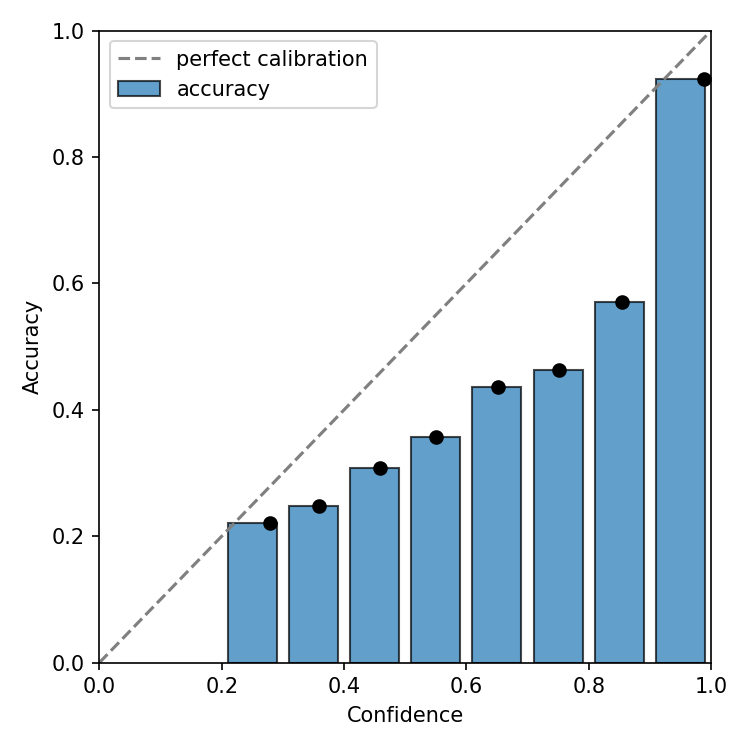
\includegraphics[width=\linewidth]{assets/bracs/tail_reliability_native.png}
    \caption{Severe, native assignment, tail classes}
  \end{subfigure}

  \vspace{0.8em}
  \begin{subfigure}[t]{0.48\linewidth}
    \centering
    
\includegraphics[width=\linewidth]{assets/bracs/tail_reliability_difficulty_aligned.png}
    \caption{Severe, aligned assignment, tail classes}
  \end{subfigure}\hfill
  \begin{subfigure}[t]{0.48\linewidth}
    \centering
    
\includegraphics[width=\linewidth]{assets/bracs/tail_reliability_difficulty_reversed.png}
    \caption{Severe, reversed assignment, tail classes}
  \end{subfigure}
  \caption{BRACS reliability curves for the balanced reference and severe-condition tail classes on the first locked partition.}
  \label{fig:reliability-bracs}
\end{figure}

\begin{figure}[ht]
  \centering
  \begin{subfigure}[t]{0.48\linewidth}
    \centering
    
\includegraphics[width=\linewidth]{assets/tcga_ut/reliability_diagram.png}
    \caption{Balanced reference, all classes}
  \end{subfigure}\hfill
  \begin{subfigure}[t]{0.48\linewidth}
    \centering
    
\includegraphics[width=\linewidth]{assets/tcga_ut/tail_reliability_native.png}
    \caption{Severe, native assignment, tail classes}
  \end{subfigure}

  \vspace{0.8em}
  \begin{subfigure}[t]{0.48\linewidth}
    \centering
    
\includegraphics[width=\linewidth]{assets/tcga_ut/tail_reliability_difficulty_aligned.png}
    \caption{Severe, aligned assignment, tail classes}
  \end{subfigure}\hfill
  \begin{subfigure}[t]{0.48\linewidth}
    \centering
    
\includegraphics[width=\linewidth]{assets/tcga_ut/tail_reliability_difficulty_reversed.png}
    \caption{Severe, reversed assignment, tail classes}
  \end{subfigure}
  \caption{TCGA-UT reliability curves for the balanced reference and severe-condition tail classes on the first locked partition. Both figure sets use ten equal-width confidence bins.}
  \label{fig:reliability-tcga}
\end{figure}



\clearpage
\section{Do Individual Partitions Change the Conclusion?}
\label{app:splits}
Equal-weight pooling is easier to interpret when the individual partitions agree. Tables~\ref{tab:per-split} and~\ref{tab:split-calibration} show every partition-specific deficit on its own endpoint scale; their averages and paired uncertainty are already reported in Appendix~\ref{app:damage-estimates}. The severity checks in Appendix~\ref{app:realized-validity} rule out large allocation-ratio variation as the explanation for these differences.

\begin{table}[H]
\centering\small\setlength{\tabcolsep}{4pt}
% Generated by assets/build_readable_appendix.mjs; do not edit.
\begin{tabular}{@{}lllrrr@{}}
\toprule
Dataset & Comparison & Assignment & Partition 1 & Partition 2 & Partition 3 \\
\midrule
BRACS & Patient shortage & Native & 2.52 & 0.75 & 5.47 \\
BRACS & Patient shortage & Aligned & 2.52 & 0.67 & 5.92 \\
BRACS & Patient shortage & Reversed & 2.00 & 0.47 & 5.39 \\
BRACS & Moderate & Native & 3.67 & 3.53 & 2.83 \\
BRACS & Moderate & Aligned & 1.63 & 2.97 & -0.12 \\
BRACS & Moderate & Reversed & 8.61 & 6.76 & 9.14 \\
BRACS & Severe & Native & 4.67 & 5.99 & 5.69 \\
BRACS & Severe & Aligned & 1.19 & 7.30 & 4.41 \\
BRACS & Severe & Reversed & 12.88 & 12.87 & 13.94 \\
BRACS & Severe spread & Native & 5.63 & 9.98 & 9.68 \\
BRACS & Severe spread & Aligned & 5.56 & 3.84 & 3.04 \\
BRACS & Severe spread & Reversed & 14.29 & 11.60 & 15.40 \\
TCGA-UT & Patient shortage & Native & 4.14 & 4.82 & 5.33 \\
TCGA-UT & Patient shortage & Aligned & 4.35 & 4.69 & 5.45 \\
TCGA-UT & Patient shortage & Reversed & 4.23 & 4.82 & 5.46 \\
TCGA-UT & Moderate & Native & 0.56 & 0.36 & 0.17 \\
TCGA-UT & Moderate & Aligned & 0.08 & 0.13 & 0.19 \\
TCGA-UT & Moderate & Reversed & 0.50 & 0.73 & 0.13 \\
TCGA-UT & Severe & Native & 1.87 & 1.66 & 1.82 \\
TCGA-UT & Severe & Aligned & 1.34 & 1.52 & 1.14 \\
TCGA-UT & Severe & Reversed & 1.40 & 1.60 & 1.35 \\
TCGA-UT & Severe spread & Native & 5.07 & 4.55 & 5.26 \\
TCGA-UT & Severe spread & Aligned & 3.05 & 2.74 & 3.44 \\
TCGA-UT & Severe spread & Reversed & 2.50 & 2.14 & 2.58 \\
\bottomrule
\end{tabular}

\caption{Balanced-accuracy deficit by partition, in percentage points. Positive means damage. Partitions 1--3 correspond to stored partition identifiers 0--2.}
\label{tab:per-split}
\end{table}
\begin{table}[H]
\centering\small\setlength{\tabcolsep}{4pt}
% Generated by assets/build_readable_appendix.mjs; do not edit.
\begin{tabular}{@{}lllrrr@{}}
\toprule
Dataset & Comparison & Assignment & Partition 1 & Partition 2 & Partition 3 \\
\midrule
BRACS & Patient shortage & Native & 0.070 & 0.171 & 0.171 \\
BRACS & Patient shortage & Aligned & 0.070 & 0.148 & 0.202 \\
BRACS & Patient shortage & Reversed & 0.060 & 0.138 & 0.204 \\
BRACS & Moderate & Native & 0.027 & 0.092 & 0.437 \\
BRACS & Moderate & Aligned & 0.598 & 0.243 & 0.298 \\
BRACS & Moderate & Reversed & 0.410 & 0.037 & 1.814 \\
BRACS & Severe & Native & 0.483 & 0.160 & 1.420 \\
BRACS & Severe & Aligned & 0.306 & 0.978 & 0.904 \\
BRACS & Severe & Reversed & 1.266 & 1.567 & 2.398 \\
BRACS & Severe spread & Native & 0.357 & 0.183 & 0.075 \\
BRACS & Severe spread & Aligned & 1.144 & 0.703 & 0.877 \\
BRACS & Severe spread & Reversed & 1.489 & 0.941 & 0.956 \\
TCGA-UT & Patient shortage & Native & 0.209 & 0.356 & 0.224 \\
TCGA-UT & Patient shortage & Aligned & 0.207 & 0.343 & 0.226 \\
TCGA-UT & Patient shortage & Reversed & 0.203 & 0.347 & 0.224 \\
TCGA-UT & Moderate & Native & -0.197 & -0.159 & -0.241 \\
TCGA-UT & Moderate & Aligned & -0.125 & -0.148 & -0.080 \\
TCGA-UT & Moderate & Reversed & -0.069 & -0.057 & -0.060 \\
TCGA-UT & Severe & Native & -0.190 & -0.187 & -0.129 \\
TCGA-UT & Severe & Aligned & 0.133 & 0.177 & 0.119 \\
TCGA-UT & Severe & Reversed & -0.011 & -0.091 & 0.010 \\
TCGA-UT & Severe spread & Native & 0.149 & 0.273 & 0.156 \\
TCGA-UT & Severe spread & Aligned & 0.224 & 0.137 & 0.236 \\
TCGA-UT & Severe spread & Reversed & 0.063 & 0.106 & 0.073 \\
\bottomrule
\end{tabular}

\caption{Tail-group NLL deficit by partition, in nats. Negative values mean improved probability quality. These partition estimates do not replace pooled patient-bootstrap inference.}
\label{tab:split-calibration}
\end{table}

\noindent BRACS balanced-accuracy damage from patient shortage is smallest in partition 2 and largest in partition 3, so two partitions carry most of the pooled magnitude. TCGA-UT repeats the pooled deficit under a stronger patient-coverage contrast. Agreement on the broad mechanism therefore coexists with substantial uncertainty about its magnitude in a particular split.

\section{What Additional Computation Was Required?}
\label{app:cost}
The useful comparison is additional cost against cross-entropy in the same condition. Tables~\ref{tab:cost} and~\ref{tab:cost-tcga} summarize each method's minimum and maximum recorded differences across assignments and conditions. Minutes denote accelerator time; MiB denotes peak memory divided by $2^{20}$. Examples are processed presentations, Unique is the recorded unique-exposure count, and Parameters is model size. These ranges describe measured variation, not uncertainty intervals; rounded zeros can hide small differences.

\begin{table}[H]
\centering\footnotesize\setlength{\tabcolsep}{3pt}
% Generated by assets/build_readable_appendix.mjs; do not edit.
\begin{tabular}{@{}>{\raggedright\arraybackslash}p{3.8cm}rrrrr@{}}
\toprule
Method & Minutes & MiB & Examples & Unique & Parameters \\
\midrule
Balanced sampling & \num{0.0} & \num{-15.9} to \num{0.0} & \num{0} & \num{-4} to \num{0} & \num{0} \\
CE + soft $F_1$ & \num{0.2} to \num{0.8} & \num{-15.9} to \num{0.0} & \num{0} & \num{-4} to \num{0} & \num{0} \\
CE + soft MCC & \num{0.1} & \num{-15.9} to \num{15.9} & \num{0} & \num{-4} to \num{0} & \num{0} \\
CFAL & \num{0.1} to \num{0.2} & \num{1037.6} to \num{1085.3} & \num{0} & \num{0} & \num{-7} \\
Nominal support & \num{0.0} & \num{-15.9} to \num{15.9} & \num{0} & \num{0} & \num{0} \\
cRT & \num{0.1} & \num{-19.3} to \num{-3.3} & \num{129} & \num{0} & \num{0} \\
Focal loss & \num{0.0} to \num{0.1} & \num{-15.9} to \num{15.9} & \num{0} & \num{0} & \num{0} \\
Independent support & \num{0.0} & \num{-0.2} to \num{0.0} & \num{0} & \num{0} & \num{0} \\
Independent support (matched $\beta$) & \num{0.0} & \num{-0.2} to \num{0.0} & \num{0} & \num{0} & \num{0} \\
Logit adjustment (train) & \num{0.0} & \num{-15.9} to \num{0.0} & \num{0} & \num{0} & \num{0} \\
OKO & \num{0.0} to \num{0.1} & \num{-16.5} to \num{31.1} & \num{2727} to \num{2983} & \num{-80} to \num{0} & \num{3591} \\
Difficulty & \num{0.0} & \num{-15.9} to \num{15.9} & \num{0} & \num{0} & \num{0} \\
Logit adjustment (post-hoc) & \num{-0.2} & \num{-3331.2} to \num{-3315.0} & \num{-577400} & \num{-19330} & \num{0} \\
Diversity & \num{0.0} to \num{0.1} & \num{-10.9} to \num{34.1} & \num{0} & \num{0} & \num{0} \\
Prevalence & \num{0.0} & \num{-15.9} to \num{15.9} & \num{0} & \num{0} & \num{0} \\
\bottomrule
\end{tabular}

\caption{BRACS additional cost against matched cross-entropy. Post-hoc adjustment records incremental work after checkpoint reuse; its negative training counts are not end-to-end savings.}
\label{tab:cost}
\end{table}
\begin{table}[H]
\centering\footnotesize\setlength{\tabcolsep}{3pt}
% Generated by assets/build_readable_appendix.mjs; do not edit.
\begin{tabular}{@{}>{\raggedright\arraybackslash}p{3.8cm}rrrrr@{}}
\toprule
Method & Minutes & MiB & Examples & Unique & Parameters \\
\midrule
Balanced sampling & \num{0.0} to \num{0.1} & \num{-15.9} to \num{0.1} & \num{0} & \num{-10} to \num{0} & \num{0} \\
CE + soft $F_1$ & \num{1.7} to \num{3.2} & \num{-15.9} to \num{15.9} & \num{0} & \num{-10} to \num{0} & \num{0} \\
CE + soft MCC & \num{0.1} to \num{0.2} & \num{-15.9} to \num{15.9} & \num{0} & \num{-10} to \num{0} & \num{0} \\
CFAL & \num{0.2} to \num{0.8} & \num{14514.9} to \num{14543.5} & \num{0} & \num{0} & \num{-30} \\
Nominal support & \num{-0.1} to \num{0.1} & \num{-15.9} to \num{15.9} & \num{0} & \num{0} & \num{0} \\
cRT & \num{0.2} to \num{0.5} & \num{-19.3} to \num{12.6} & \num{43} & \num{0} & \num{0} \\
Focal loss & \num{0.0} to \num{0.2} & \num{-15.9} to \num{0.0} & \num{0} & \num{0} & \num{0} \\
Independent support & \num{-0.1} to \num{0.1} & \num{-15.9} to \num{15.9} & \num{0} & \num{0} & \num{0} \\
Independent support (matched $\beta$) & \num{-0.1} to \num{0.1} & \num{-15.9} to \num{0.1} & \num{0} & \num{0} & \num{0} \\
Logit adjustment (train) & \num{-0.2} to \num{0.1} & \num{-15.9} to \num{31.8} & \num{0} & \num{0} & \num{0} \\
OKO & \num{0.2} to \num{0.4} & \num{-16.5} to \num{15.2} & \num{396} to \num{524} & \num{-21} to \num{0} & \num{15390} \\
Difficulty & \num{-0.1} to \num{0.2} & \num{-15.9} to \num{15.9} & \num{0} & \num{0} & \num{0} \\
Logit adjustment (post-hoc) & \num{-0.7} to \num{-0.5} & \num{-18024.4} & \num{-1340000} & \num{-44660} & \num{0} \\
Diversity & \num{0.0} to \num{0.2} & \num{-14.0} to \num{37.8} & \num{0} & \num{0} & \num{0} \\
Prevalence & \num{0.0} to \num{0.1} & \num{-15.9} to \num{0.0} & \num{0} & \num{0} & \num{0} \\
\bottomrule
\end{tabular}

\caption{TCGA-UT additional cost, with the same units and aggregation as Table~\ref{tab:cost}. Exposure differences and memory overhead vary by mechanism.}
\label{tab:cost-tcga}
\end{table}

\noindent Exposure matching removes most differences in data volume, while integral update counts leave residual mismatches for methods such as OKO and two-stage classifier retraining. CFAL has substantially higher peak memory than cross-entropy in both datasets. Post-hoc logit adjustment reuses a trained checkpoint, so its incremental training cost cannot be compared with a complete training run without including that checkpoint's cost. These distinctions are more informative than a single universal ranking of computational expense.


\clearpage
\bibliographystyle{plainnat}
\bibliography{references}

\end{document}
